%---------------------------------------------------------------------------------
\chapter{NOMA-Aided Multi-UAV Communications in Full-Duplex Heterogeneous Networks}
\label{chap:NOMA_aided_multi_UAV_FD_HetNet}
%---------------------------------------------------------------------------------

\section{Introduction}

Apart from FD-based HBD-UCSs, one can also consider power-domain NOMA as a means to further improve spectrum efficiency in UAV communications. The concept of NOMA hinges on the fact that nodes in NOMA-aided systems are multiplexed in the power-domain to share the same spectrum. In contrast, conventional orthogonal multiple access schemes employ orthogonal allocation of time-frequency resource blocks for each node in the network. Thus, compared to orthogonal multiple access systems, NOMA-aided systems are capable of achieving higher spectrum utilization. When adopted for multi-UAV communications, superposition coding is employed to enforce unequal power allocation for all UAVs and GSs. Thereafter, the desired messages are recovered at the receivers via SIC when the interference is stronger than the desired message \cite{liu2019uav,yang2016general,cui2016novel,kader2018full,salehi2019meta,weber2007transmission,islam2017power}. For receivers experiencing weak interference, the desired message is simply detected by treating interference as noise \cite{liu2019uav,islam2017power}.\footnote{The work in this chapter is derived from \cite{ernest2019hetnet}, which has been submitted for publication.}

Already, NOMA has been investigated as a means to improve spectrum efficiency in heterogeneous networks (HetNets) for cellular communications \cite{moltafet2018optimal,liu2018heterogeneous} and UAV communications \cite{liu2019dsf}. Although promising, the orthogonal allocation of time-frequency resources is still necessary as power-domain multiplexing is only employed during UL or DL transmissions \cite{ernest2019noma,ding2018coexistence}. 

To further address spectrum scarcity, one can consider integrating NOMA-aided multi-UAV communications into FD HetNets, i.e., FD-HetNets, comprising FD-capable GSs (FD-GSs) and HD macro base stations (MBSs). In particular, implementing NOMA-aided multi-UAV communications in FD-HetNets enable UL UAVs and DL UAVs, equipped with conventional HD transceivers, to simultaneously operate on the same spectrum thanks to the operation of FD-GSs. As compared to conventional NOMA-aided HD-HetNets, where all nodes operate in HD mode, higher spectrum efficiency can be attained via NOMA-aided FD-HetNets. However, such FD-based systems are also impaired by residual SI due to carrier phase noise and imperfect SI channel estimation \cite{sahai2013impact}, and interference from UL UAVs \cite{tan2018joint,ernest2019noma,ernest2019power}.

\subsection{Related Literature}
Despite being limited by residual SI and UL interference, NOMA-aided FD-HetNets have started receiving interest in the literature as a potential solution to address spectrum scarcity. For instance, a power control technique was proposed in \cite{lei2018noma} for interference management in a NOMA-aided FD-HetNet, with similar works on NOMA-aided HD-HetNets \cite{moltafet2018optimal,liu2018heterogeneous} noted. For UAV communications in FD-HetNets and HD-HetNets, there exists limited studies in the literature. To illustrate, resource allocation and UAV placement in HD-HetNets were investigated in \cite{liu2019dsf} and \cite{sharma2016uavs}, respectively, while \cite{zhang20183} and \cite{zhang2018number} analyzed the placement of aerial BSs for FD-HetNets. From the above studies, an analysis of NOMA-aided multi-UAV communications in FD-HetNets is, to the best of our knowledge, unavailable in the literature. Although there exists some works on NOMA-aided FD-HetNets and NOMA-aided HD-HetNets in cellular networks, the conclusions from those studies may not be readily applied for multi-UAV communications due to differences in operating environments and deployment constraints between cellular and multi-UAV systems.

One such difference is the channel model for both cellular and UAV communications. In cellular communications, Rayleigh fading \cite{ding2018coexistence} and Nakagami-$m$ fading \cite{chu2018performance,hou2018multiple} are commonly assumed. However, apart from UAV communications taking place over Rayleigh fading \cite{zhao2019joint,mei2019uplink} and Nakagami-$m$ fading \cite{chetlur2017downlink}, other types of fading can also be encountered. For instance, transmissions over Rician fading channels have been noted for UAV-to-GS links \cite{matolak2017air_suburban,matolak2017air_water,sun2017air_hilly,tan2018joint,ernest2019noma,ernest2019power,nasir2019uav,nguyen2018novel} and UAV-to-UAV links \cite{tan2018joint,ernest2019power,yuan2018capacity}.

Another difference stems from the spatial distribution of nodes in cellular and UAV communications. As discussed earlier, the application of UAVs in future wireless networks has garnered intense interest in deploying UAV-aided wireless connectivity via aerial BSs or relays. \textcolor{black}{Hence, the spatial location and mobility of the UAVs  need to be accounted for before any accurate performance evaluation}. To accomplish such a feat, one can employ the useful tools of stochastic geometry for multi-UAV networks. A common technique seen in the literature involves modeling the spatial location of UEs as a PPP. However, it has since been shown in \cite{chetlur2017downlink} that the PPP model is unsuitable for multi-UAV networks, as the number of deployed UAVs is usually fixed. Such an instance can be illustrated when UAVs function as aerial BSs in a given region \cite{chetlur2017downlink,wang2018modeling}. In such scenarios, the homogeneous BPP can be used to provide an accurate modeling of the UAV spatial locations \cite{chetlur2017downlink,wang2018modeling}. In spite of several studies that have analyzed multi-UAV networks using the BPP model, e.g., \cite{chetlur2017downlink,wang2018modeling,enayati2019moving}, similar studies involving NOMA-aided multi-UAV communications in FD-HetNets are lacking in the literature.

Based on the above discussions, an ergodic capacity analysis of NOMA-aided multi-UAV communications in a FD-HetNet is conducted in this chapter. By considering Rician fading channels and the BPP model for UAV spatial location modeling, we demonstrate the feasibility and advantages of NOMA-aided multi-UAV communications in FD-HetNets in a realistic setting. 

%%%%%%%%%%%%%%%%%%%%%%%%%%%%%%%%%%%%%%%%%%%%%%%%%%%%%%%%%%%%%%%%%%%%%%%%%%%%%%%%%%%%%%%%%%%%%%%%%%%%%%%%%%%%%%%%%%%%%%%%%%%%%%%%%%%%%%%%%
% Section 2 : System Model
\section{System Model} \label{NOMA_aided_multi_UAV_FD_HetNet_sec_sys_model}
\begin{figure} [tpb]
\centering
\vspace{-0.7cm}
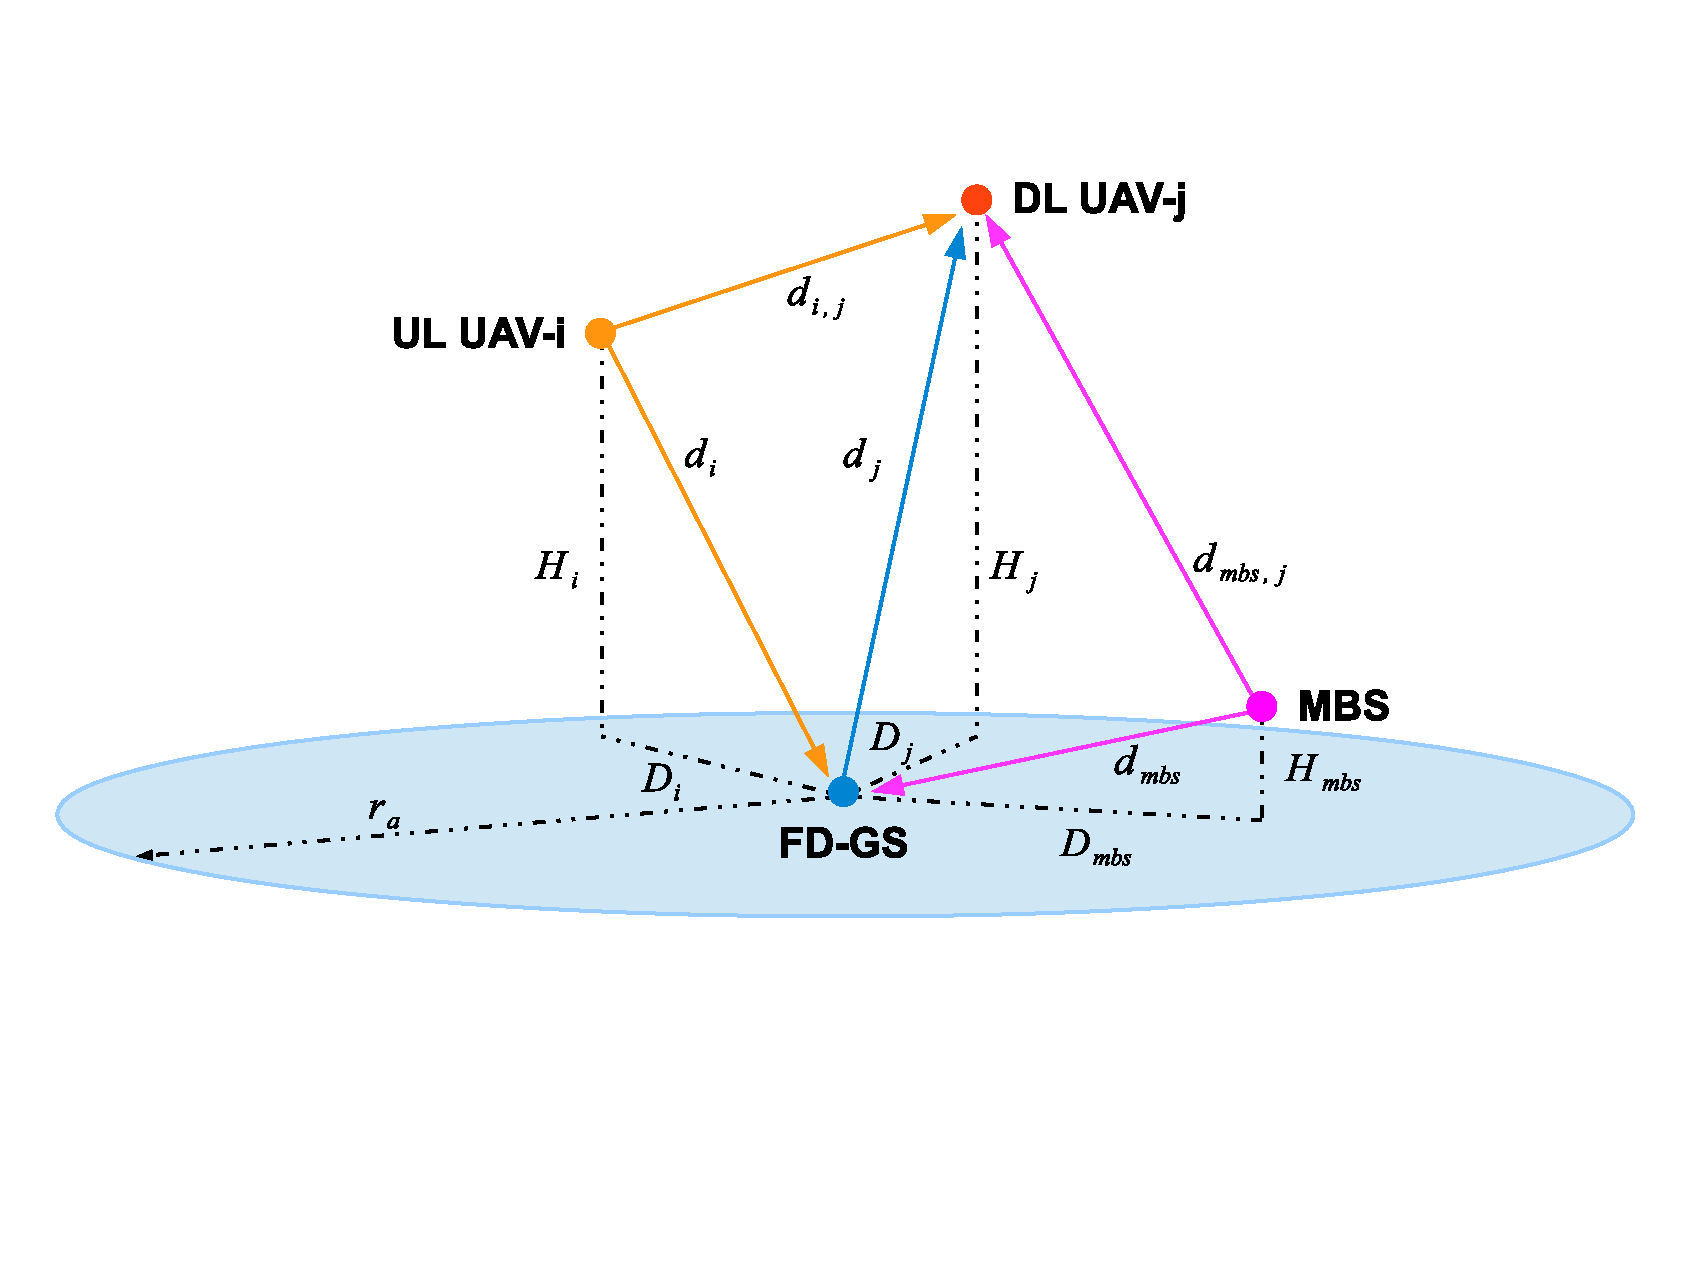
\includegraphics [width=0.6\columnwidth]{chap7_fig/block_diagram3.eps} 
\vspace{-2cm}
\caption{The FD-HetNet for NOMA-aided multi-UAV communications is illustrated here. The FD-GS in the FD-HetNet enables HD uplink and downlink UAVs and the HD MBS to concurrently share the same spectrum for NOMA transmissions. Through the BPP, it is assumed that the spatial locations of the deployed UAVs and the MBS follow a uniform distribution around a disc, with origin $O$ at the FD-GS and radius $r_a$.}
\label{fig:NOMA_aided_multi_UAV_FD_HetNet_block_diagram}
%\vspace{-0.3in}
\end{figure}

Consider a FD-HetNet supporting NOMA-aided multi-UAV communications in a suburban environment (Fig. \ref{fig:NOMA_aided_multi_UAV_FD_HetNet_block_diagram}). The FD-HetNet comprises $N_{U}$ HD single-antenna UL UAVs, $N_D$ HD single-antenna DL UAVs, one HD single-antenna MBS, and a FD-GS. The FD-GS is assumed to be operating with one antenna each for signal transmission and reception. It is also assumed that the FD-GS receives uplink data from the $N_{U}$ UL UAVs and MBS-to-GS data from the MBS while concurrently transmitting DL data to the $N_D$ DL UAVs on the same spectrum through power-domain NOMA.\footnote{It is worth noting that such a system model has been studied in \cite{zhang20183} and \cite{zhang2018number} in the context of aerial BSs.} Due to FD transmissions at the GS, the DL UAVs experience interference from the MBS and UL UAVs \cite{tan2018joint,ernest2019outage}, as well as MUI from other DL UAVs \cite{ernest2019noma}. In this regard, the DL UAVs are assumed to be equipped with imperfect SIC detectors. For the FD-GS, SI mitigation is assumed and only residual SI is considered to account for FD transceiver impairments \cite{ernest2019hybrid,tan2018joint,ernest2019outage,sahai2013impact}. Finally, it is assumed that the suburban UAV channel undergoes Rician fading \cite{matolak2017air_suburban}, with compensated Doppler shift assumed in this chapter \cite{tan2018joint,ernest2019outage}. Rician fading is also assumed for the SI channel at the FD-GS to account for SI mitigation \cite{tan2018joint,ernest2019outage, ernest2019hybrid}. A summary of important notations is given in Table \ref{table:NOMA_aided_multi_UAV_FD_HetNet_summary_impt_notations}.

\subsection{Distance Distribution of the UAVs and MBS}

Inspired by the studies in \cite{chetlur2017downlink, wang2018modeling, ernest2019hybrid}, the spatial locations of the UL UAVs, DL UAVs and the MBS are assumed to follow a BPP. Let the UL UAVs and DL UAVs be indexed by $1 \leq i \leq N_U$ and $1 \leq j \leq N_D$, respectively. Then, we denote $H_i = H_{min} + \omega \frac{i}{N_U}$ and $H_j = H_{min} + \omega \big[ 1+\frac{i}{N_D} \big]$ as the respective altitudes (km) of UL UAV-$i$ and DL UAV-$j$, where $\omega>0$ indicates the altitude separation factor between the UL and DL UAVs, $H_{min}$ denotes a minimum altitude such that $0<H_{mbs}<H_{min}$, and $H_{mbs}$ is the height of the MBS antenna.

Based on the BPP assumption, let the spatial location of the UL UAVs, DL UAVs, and MBS be uniformly distributed around a disc with origin $O$ at the FD-GS, radius $r_a$, and angle $\left[0,2\pi\right)$ \cite{chetlur2017downlink,ernest2019hybrid}. The Euclidean distances (km) from the FD-GS to the MBS, UL UAV-$i$, and DL UAV-$j$ are denoted as $d_{mbs}$, $d_{i}$, and $d_{j}$, respectively. For $x \in \{i,j,mbs\}$, the Euclidean distance $d_x$ is defined as $d_{x} = \sqrt{D_{x}^2 + H_{x}^2}$, where $D_{x}$ is the Euclidean distance between the projection of node-$x$ onto the ground plane and the FD-GS. Finally, the inter-UAV distance between UL UAV-$i$ and DL UAV-$j$ is defined as $d_{i,j}$ while the distance between the MBS and DL UAV-$j$ is denoted as $d_{mbs,j}$.

The PDF of $d_x$ is given as \cite[eq. (3)]{chetlur2017downlink}:
%%%%%%%%%%%%%%%%%%%%%%%%%%%%%%%%%%%%%%%%%%%%%%%%%%%%%%%%%%%%%%%%%%%%%%%%%%%%%%%%%
\begin{eqnarray}
f_{d_{x}}(w_x) &=&  \frac{2w_x}{r_a^2}_,
\end{eqnarray}
%%%%%%%%%%%%%%%%%%%%%%%%%%%%%%%%%%%%%%%%%%%%%%%%%%%%%%%%%%%%%%%%%%%%%%%%%%%%%%%%%
where $x \in \{i,j,mbs\}$, $L_{m,x} \leq w_{x} \leq L_{p,x}$, $L_{m,x} = H_{x}$, and $L_{p,x} = \sqrt{H_x+r_{a}^2}$. 

For the inter-UAV distance ($d_{i,j}$) and the distance between the MBS and DL UAV-$j$ ($d_{mbs,j}$), the conditional PDF $f_{d_{x,j}}(w|d_{j}), x \in \{i,mbs\}$ is defined as \cite[eq. (2)]{chetlur2017downlink}, \cite[eq. (1)]{ernest2019hybrid}:
%%%%%%%%%%%%%%%%%%%%%%%%%%%%%%%%%%%%%%%%%%%%%%%%%%%%%%%%%%%%%%%%%%%%%%%%%%%%%%%%%
\begin{eqnarray}
f_{d_{x,j}}(w|d_{j}) \hspace{-0.1cm} = \hspace{-0.1cm} \begin{cases}
    \hspace{1cm} \frac{2w}{r_a^2} \hspace{3.3cm}, H_{x,j} \leq w \leq L_{q,x}\\
    \hspace{-0.1cm} \frac{2w}{\pi r_a^2}\arccos\left( \frac{w^2 + d_{j}^2 - \big(r_a^2+H_{x,j}^2\big)}{2d_{j}\sqrt{w^2 - H_{x,j}^2}} \right), L_{q,x} < w \leq L_{r,x}\\ 
  \end{cases}\hspace{-1cm} \\\nonumber
\end{eqnarray}
%%%%%%%%%%%%%%%%%%%%%%%%%%%%%%%%%%%%%%%%%%%%%%%%%%%%%%%%%%%%%%%%%%%%%%%%%%%%%%%%%
where $L_{q,x}=\sqrt{\big(r_a - d_{j}\big)^2 + H_{x,j}^2}$, $L_{r,x}=\sqrt{\big(r_a + d_{j}\big)^2 + H_{x,j}^2}$, $H_{i,j} = H_j - H_i$ is the separation altitude between UL UAV-$i$ and DL UAV-$j$, and $H_{mbs,j} = H_j - H_{mbs}$ is the altitude between the MBS and DL UAV-$j$.

Through the PDFs, $f_{d_{x}}(w)$ and $f_{d_{x,j}}(w|d_{j})$, a performance analysis of NOMA-aided multi-UAV communications in the FD-HetNet  can be obtained with the spatial locations of the UAVs and MBS taken into consideration. 

\subsection{Instantaneous SINR at the FD-GS}

To detect the messages transmitted by both the MBS and UL UAVs at the FD-GS, an SIC detection process is employed.\footnote{By extension, it is assumed that the FD-GS has prior knowledge of the locations of the MBS and all UAVs. For the latter, such information can be obtained from flight plans approved by relevant authorities.} In particular, the FD-GS performs SIC to detect and remove the MBS SOI from the received composite signal. The FD-GS then detects the SOI from the UL UAVs, starting with UL UAV-1, in the presence of MUI \cite{cui2016novel,kader2018full,salehi2019meta,weber2007transmission,islam2017power}. The SIC detection process is repeated until the SOIs of all the remaining UL UAVs are detected.

% cite commun letts.
Let $X_{mbs}$, $X_i$, and $Y_{si,1}$ be non-centered Chi-squared distributed RVs with respective Rician $K$ factors $K_{mbs}$, $K_i$, and $K_{si,1}$. Also, let $Y_{si,2}$ be an exponentially distributed RV. Then, the instantaneous SINR to detect the SOI of the MBS at the FD-GS $\Big(SINR_{mbs}^{FD}\Big)$ is:
%%%%%%%%%%%%%%%%%%%%%%%%%%%%%%%%%%%%%%%%%%%%%%%%%%%%%%%%%%%%%%%%%%%%%%%%%%%%%%%%%
\begin{eqnarray} \label{NOMA_aided_multi_UAV_FD_HetNet_fd_noma_mbs_sinr}
SINR_{mbs}^{FD} = \frac{ \rho d_{mbs}^{-n} X_{mbs}}{1 + \rho \sum_{i=1}^{N_U} d_i^{-n} X_{i} + \rho_{si} Y_{si,1} + \rho_{si}  Y_{si,2}}_,
\end{eqnarray}
%%%%%%%%%%%%%%%%%%%%%%%%%%%%%%%%%%%%%%%%%%%%%%%%%%%%%%%%%%%%%%%%%%%%%%%%%%%%%%%%%
where $n$ is the pathloss exponent, $\rho  \propto \frac{P_t}{G\sigma^2}$ is the normalized transmit power \cite{ernest2019outage}, $P_t$ is the transmit power, $G = \big(\frac{4 \pi \cdot 10^9}{3 \cdot 10^8} f_c\big)^2$, $f_c$ is the carrier frequency (MHz), $\sigma^2 = -174 + 10\log_{10}(B_W)$ is the strength of the AWGN in dBm \cite{hou2019exploiting}, $B_W$ is the bandwidth (Hz), $\rho_{si}  = P_{si} /\sigma^2$ is the normalized power of the SI, $P_{si} = P_t$ denotes the received power of the SI, $X_{mbs} = |h_{mbs}|^2$, $X_{i} = |h_{i}|^2$, $h_{mbs}$ is the channel between the FD-GS and the MBS, and $h_{i}$ is the channel between the FD-GS and UL UAV-$i$. Also, $Y_{si,1} = \epsilon |\widetilde{h}_{si}|^2$ and $Y_{si,2} = \gamma_{\phi}^2 |h_{si}|^2$, where $\widetilde{h}_{si}=h_{si}-\widehat{h}_{si}$ is the error of the imperfect SI channel gain estimate, $\widehat{h}_{si}$ is the imperfect estimation of the SI channel gain, and $\gamma_{\phi}^2$ is the strength of the Gaussian distributed phase noise \cite{sahai2013impact}.\footnote{The phase noise term $\gamma_{\phi}$ reflects the jitter effect in oscillators due to hardware imperfections \cite{sahai2013impact}.} The SI channel estimation error ($\widetilde{h}_{si}$) is modeled as a circularly symmetric zero-mean complex Gaussian RV with variance $\epsilon$ to account for the worst case residual SI, \cite{tan2018joint,ernest2019outage,zlatanov2017capacity}. In this way, the total amount of SI suppression to bring the residual SI signal below the noise floor $(\sigma^2)$ is calculated as $1 / (\epsilon\sigma^2)$ \cite{ernest2019outage}. 

Similarly, the instantaneous SINR to detect the SOI of the UL UAVs at the FD-GS $\Big(SINR_{i}^{FD}\Big)$ is:
%%%%%%%%%%%%%%%%%%%%%%%%%%%%%%%%%%%%%%%%%%%%%%%%%%%%%%%%%%%%%%%%%%%%%%%%%%%%%%%%%
\begin{eqnarray} \label{NOMA_aided_multi_UAV_FD_HetNet_fd_noma_uav_i_sinr}
SINR_{i}^{FD} = \frac{ \rho  d_{i}^{-n} X_i}{1 + \sum_{k=i+1}^{N_U} \rho  d_k^{-n} Y_k + \rho_{si}  Y_{si,1} + \rho_{si}  Y_{si,2}}_,
\end{eqnarray}
%%%%%%%%%%%%%%%%%%%%%%%%%%%%%%%%%%%%%%%%%%%%%%%%%%%%%%%%%%%%%%%%%%%%%%%%%%%%%%%%%
where $Y_{k} = |h_k|^2$ is a non-centered Chi-squared distributed RV with Rician $K$ factor $K_k$, and $h_k$ is the channel between the FD-GS and the remaining UL UAVs.

\begin{table}[]
\centering
\caption{Summary of Important Notations}
\label{table:NOMA_aided_multi_UAV_FD_HetNet_summary_impt_notations} 
\scalebox{0.8}{
\begin{tabular}{ll}
\hline
\textbf{Notations}		& \textbf{Description}																	\\  \hline \hline
$1 \leq i \leq N_U$		& Index of UL UAV-$i$																		\\
$1 \leq j \leq N_D$		& Index of DL UAV-$j$																		\\ \hline
$H_{min}$; $\omega$		&	Minimum UAV altitude; Altitude separation factor			\\
$H_{i}$; $H_{j}$			&	Altitude of UL UAV-$i$;	Altitude of DL UAV-$j$				\\
$H_{mbs}$							& MBS antenna height																		\\
$H_{i,j}$							&	Altitude between UL UAV-$i$ and DL UAV-$j$						\\
$H_{mbs,j}$						&	Altitude between the MBS and DL UAV-$j$								\\ \hline
$d_{mbs}$							& Euclidean distance between the FD-GS and the MBS			\\
$d_{i}$								& Euclidean distance between the FD-GS and UL UAV-$i$		\\
$d_{j}$								& Euclidean distance between the FD-GS and DL UAV-$j$		\\
$d_{mbs,j}$						& Euclidean distance between the MBS and DL UAV-$j$			\\
$d_{i,j}$							& Euclidean distance between UL UAV-$i$ and DL UAV-$j$	\\ \hline
$P_t$; $\rho$					& Transmit power; Normalized transmit power							\\
$P_{si}$; $\rho_{si}$	& Received power of the SI; Normalized SI power					\\
$\sigma^2$						& Strength of AWGN																			\\
$\epsilon$						& SI channel estimation error	at the FD-GS							\\
$\gamma_{\phi}^2$			& Strength of phase noise at the FD-GS oscillator				\\
$\beta_{mbs,j}$				& Residual interference from the MBS at DL UAV-$j$ 			\\
$\beta_{i,j}$					& Residual interference from UL UAV-$i$ at DL UAV-$j$ 	\\
$\alpha_j$						& NOMA power allocation factor for DL UAV-$j$						\\ \hline
\end{tabular}}
\end{table}
%A summary of important notations is also given in Table \ref{table:HBD_multi_UAV_summary_impt_notations}.

\subsection{Instantaneous SINR at Downlink UAV-$j$}

At DL UAV-$j$, an SIC detector is employed to detect the SOI transmitted by the FD-GS. In particular, the SIC detector at DL UAV-$j$ detects the SOI in the presence of MUI from the other DL UAVs, as well as interference from both the UL UAVs and MBS.\footnote{Similar to the FD-GS, it is assumed that all DL UAVs have prior knowledge of the locations of the FD-GS, MBS and surrounding UAVs.}

Let $X_{j}$, $Y_{mbs,j}$, and $Y_{i,j}$ be non-centered Chi-squared distributed random variables RVs with respective Rician $K$ factors $K_{i}$, $K_{mbs,j}$, and $K_{i,j}$. Then, the instantaneous SINR $\Big(SINR_j^{FD}\Big)$ at DL UAV-$j$ is:
%%%%%%%%%%%%%%%%%%%%%%%%%%%%%%%%%%%%%%%%%%%%%%%%%%%%%%%%%%%%%%%%%%%%%%%%%%%%%%%%%
\begin{eqnarray} \label{NOMA_aided_multi_UAV_FD_HetNet_fd_noma_uav_j_sinr}
SINR_j^{FD} & = & \frac{\rho  \alpha_j d_j^{-n} X_j}{1 + \rho  d_{mbs,j}^{-n} Y_{mbs,j} +  \rho  d_j^{-n} X_j \sum_{k=1}^{j-1}\alpha_k + \rho  \sum_{i=1}^{N_U} d_{i,j}^{-n} Y_{i,j}}_,
\end{eqnarray}
%%%%%%%%%%%%%%%%%%%%%%%%%%%%%%%%%%%%%%%%%%%%%%%%%%%%%%%%%%%%%%%%%%%%%%%%%%%%%%%%%
where $X_j = |h_j|^2$, $Y_{mbs,j} = \beta_{mbs,j}|h_{mbs,j}|^2$, $Y_{i,j} = \beta_{i,j} |h_{i,j}|^2$, $h_{j}$ is the channel between the FD-GS and DL UAV-$j$, $h_{mbs,j}$ is the channel between the MBS and DL UAV-$j$, $h_{i,j}$ is the channel between UL UAV-$i$ and DL UAV-$j$, and $\alpha_j$ is the power allocation factor for DL UAV-$j$ such that $\sum_{j=1}^{N_D} \alpha_j = 1$. Also, $0 \leq \beta_{x,j} \leq 1, x \in \{mbs,i\}$ is the strength of the residual interference after SIC \cite{wang2017sir,kader2018coordinated,kader2018full,im2019outage}. 

As the DL UAVs are deployed at different altitudes, i.e., $H_{j} < H_{j+1}$, the power allocation factor $\alpha_j$ can be heuristically defined based on the altitudes of the $N_D$ DL UAVs to ensure fairness. In particular, the power allocation factor $\alpha_j$ can be defined as:
%%%%%%%%%%%%%%%%%%%%%%%%%%%%%%%%%%%%%%%%%%%%%%%%%%%%%%%%%%%%%%%%%%%%%%%%%%%%%%%%%
\begin{eqnarray}
\alpha_j & = & \frac{H_j}{\sum_{k=1}^{N_U} H_k}_,
\end{eqnarray}
%%%%%%%%%%%%%%%%%%%%%%%%%%%%%%%%%%%%%%%%%%%%%%%%%%%%%%%%%%%%%%%%%%%%%%%%%%%%%%%%%
so that DL UAVs that are further away from the FD-GS are assigned higher transmit powers \cite{liu2018heterogeneous}, i.e., $\alpha_j < \alpha_{j+1}$. In this way, DL UAV-$j$ recovers the SOI by performing SIC to remove MUI from DL UAV-$m$ for $m>j$, while ignoring MUI from DL UAV-$k$ for $k<j$ \cite{salehi2019meta,islam2017power}.

% Section : Ergodic Capacity Derivations
\section{Ergodic Capacity Derivations} \label{NOMA_aided_multi_UAV_FD_HetNet_sec_erg_cap}

In this section, ergodic capacity expressions are presented for NOMA-aided multi-UAV communications in the FD-HetNet. The UL and DL ergodic capacity expressions for NOMA-aided multi-UAV communications in a HD-HetNet are also presented as a benchmark. 

The ergodic capacity expressions presented in this section are derived based on the work in \cite[Lemma 1]{hamdi2010useful}, where a technique was proposed that enables the ergodic capacity calculation of instantaneous SINRs with both uncorrelated and correlated RVs. The present approach extends this method to evaluate the ergodic capacities of multi-UAV communications in FD-HetNets and HD-HetNets within a stochastic geometry framework.

%%%%%%%%%%%%%%%%%%%%%%%%%%%%%%%%%%%%%%%%%%%%%%%%%%%%%%%%%%%%%%%%%%%%%%%%%%%%%%%%%%%%%%%%%%%%%%%%%%%%%%%%%%%%%%%%%%%%%%%%%%%%%%%%%%%%%%%%%
\subsection{Ergodic Capacity of the MBS in the NOMA-Aided FD-HetNet}

The MBS ergodic capacity is defined as $\mathcal{C}_{mbs}^{FD} = E\Big\{\ln\Big(1+SINR_{mbs}^{FD}\Big)\Big\}$, where $E\{\bullet\}$ denotes the statistical expectation operator. To evaluate $\mathcal{C}_{mbs}^{FD}$, one has to employ calculations involving $(2N_U + 4)$-fold numerical integrations to average the PDFs of the associated RVs in $SINR_{mbs}^{FD}$. To avoid such highly intensive computations, one can instead invoke the method proposed in \cite{hamdi2010useful} that enables a simple evaluation of ergodic capacity. 

In the next theorem, we present an exact expression for $\mathcal{C}_{mbs}^{FD}$ obtained using the technique in \cite{hamdi2010useful}.

\begin{theorem} \label{NOMA_aided_multi_UAV_FD_HetNet_theorem_erg_cap_fd_noma_mbs}
%%%%%%%%%%%%%%%%%%%%%%%%%%%%%%%%%%%%%%%%%%%%%%%%%%%%%%%%%%%%%%%%%%%%%%%%%%%%%%%%%
The ergodic capacity of the MBS in the FD-HetNet is:
\begin{eqnarray} \label{NOMA_aided_multi_UAV_FD_HetNet_fd_noma_mbs}
\mathcal{C}_{mbs}^{FD} & \hspace{-0.0cm} = & \hspace{-0.0cm} \int_{L_{m,mbs}}^{L_{p,mbs}} \int_{0}^{\infty} \frac{\exp(-z)}{z} \Bigg(1-M_{X_{mbs}}\Big(z\rho  w_{mbs}^{-n}\Big)\Bigg) \nonumber \\
 & & \hspace{0cm} \times \Bigg( \prod_{i=1}^{N_U} \tau_i\big(z\rho\big) \Bigg) M_{Y_{si,1}}\big(z\rho_{si}\big) M_{Y_{si,2}}\big(z\rho_{si} \big) f_{d_{mbs}}(w_{mbs}) {dz dw_{mbs}}_,
\end{eqnarray}
%%%%%%%%%%%%%%%%%%%%%%%%%%%%%%%%%%%%%%%%%%%%%%%%%%%%%%%%%%%%%%%%%%%%%%%%%%%%%%%%%
where $M_{X}(z)$ is the moment generating function (MGF) of the non-centered Chi-squared distributed RV $X$, with Rician $K$ factor $K_X$, which is given as \cite[Table. I]{hasna2003performance}:
%%%%%%%%%%%%%%%%%%%%%%%%%%%%%%%%%%%%%%%%%%%%%%%%%%%%%%%%%%%%%%%%%%%%%%%%%%%%%%%%%
\begin{eqnarray} 
M_{X}(z) & = & \frac{1+K_X}{1+K_X+z}\exp\bigg(\frac{-K_X z}{1+K_X+z}\bigg)_,
\end{eqnarray}
%%%%%%%%%%%%%%%%%%%%%%%%%%%%%%%%%%%%%%%%%%%%%%%%%%%%%%%%%%%%%%%%%%%%%%%%%%%%%%%%%
and the function $\tau_i\big(z\rho\big)$ is defined as: 
%%%%%%%%%%%%%%%%%%%%%%%%%%%%%%%%%%%%%%%%%%%%%%%%%%%%%%%%%%%%%%%%%%%%%%%%%%%%%%%%%
\begin{eqnarray} 
\tau_i\big(z\rho\big) & = & \int_{L_{m,i}}^{L_{p,i}} M_{X_i}\Big(z\rho w_i^{-n}\Big) f_{d_i}(w_i) {dw_i}_,
\end{eqnarray}
%%%%%%%%%%%%%%%%%%%%%%%%%%%%%%%%%%%%%%%%%%%%%%%%%%%%%%%%%%%%%%%%%%%%%%%%%%%%%%%%%
which averages the MGF $M_{Y_i}\Big(z\rho w_i^{-n}\Big)$ of interfering UL UAV-$i$ with the PDF $f_{d_i}(w_i)$.
\end{theorem}
\begin{proof}
The proof is provided in Appendix \ref{NOMA_aided_multi_UAV_FD_HetNet_theorem_erg_cap_fd_noma_mbs_proof}.
\end{proof}
%%%%%%%%%%%%%%%%%%%%%%%%%%%%%%%%%%%%%%%%%%%%%%%%%%%%%%%%%%%%%%%%%%%%%%%%%%%%%%%%%

The expression in (\ref{NOMA_aided_multi_UAV_FD_HetNet_fd_noma_mbs}) enables $\mathcal{C}_{mbs}^{FD}$ to be evaluated at finite $P_t$, i.e., $\rho$, regimes, in the presence of receiver noise and interference, using $(N_U + 2)$-fold numerical integration. In contrast, a direct evaluation of $\mathcal{C}_{mbs}^{FD}$ will require $(2N_U + 4)$-fold numerical integrations. 

From (\ref{NOMA_aided_multi_UAV_FD_HetNet_fd_noma_mbs}), it is noted that $\mathcal{C}_{mbs}^{FD}$ is largely limited by the number of interfering UL UAVs $(N_U)$ and the strength of the residual SI, i.e., $\epsilon$ and $\gamma_{\phi}^2$. Thus, the ergodic capacity of the MBS at asymptotic $P_t$ regimes, i.e., $\mathcal{C}_{mbs,\infty}^{FD}$, can be obtained from (\ref{NOMA_aided_multi_UAV_FD_HetNet_fd_noma_mbs}) as shown in the following corollary.

\begin{corollary} \label{NOMA_aided_multi_UAV_FD_HetNet_corollary_erg_cap_fd_noma_mbs}
%%%%%%%%%%%%%%%%%%%%%%%%%%%%%%%%%%%%%%%%%%%%%%%%%%%%%%%%%%%%%%%%%%%%%%%%%%%%%%%%%
The asymptotic ergodic capacity of the MBS in the FD-HetNet is:
\begin{eqnarray} \label{NOMA_aided_multi_UAV_FD_HetNet_fd_noma_mbs_asymp}
\mathcal{C}_{mbs,\infty}^{FD} & \hspace{-0.2cm} = & \hspace{-0.2cm} \int_{L_{m,mbs}}^{L_{p,mbs}} \int_{0}^{\infty} \frac{1}{z} \Bigg(1-M_{X_{mbs}}\Big(z w_{mbs}^{-n}\Big)\Bigg) \Bigg( \prod_{i=1}^{N_U} \tau_i(z) \Bigg) \nonumber \\
 & & \hspace{0cm} \times  M_{Y_{si,1}}(z) M_{Y_{si,2}}(z) f_{d_{mbs}}(w_{mbs}) {dz dw_{mbs}}_.
\end{eqnarray}
%%%%%%%%%%%%%%%%%%%%%%%%%%%%%%%%%%%%%%%%%%%%%%%%%%%%%%%%%%%%%%%%%%%%%%%%%%%%%%%%%
\end{corollary}
\begin{proof}
At asymptotic $P_t$ regimes, $SINR_{mbs}^{FD}$ in (\ref{NOMA_aided_multi_UAV_FD_HetNet_fd_noma_mbs_sinr}) reduces to the following instantaneous signal-to-interference ratio (SIR), i.e., $SIR_{mbs}^{FD}$:
%%%%%%%%%%%%%%%%%%%%%%%%%%%%%%%%%%%%%%%%%%%%%%%%%%%%%%%%%%%%%%%%%%%%%%%%%%%%%%%%%
\begin{eqnarray} \label{NOMA_aided_multi_UAV_FD_HetNet_fd_noma_mbs_sir}
SIR_{mbs}^{FD} & = & \frac{d_{mbs}^{-n} X_{mbs}}{\sum_{i=1}^{N_U} d_i^{-n} X_{i} + Y_{si,1} + Y_{si,2}}_.
\end{eqnarray}
%%%%%%%%%%%%%%%%%%%%%%%%%%%%%%%%%%%%%%%%%%%%%%%%%%%%%%%%%%%%%%%%%%%%%%%%%%%%%%%%%

Then, evaluating $\mathcal{C}_{mbs,\infty}^{FD} = E\Big\{\ln\Big(1+SIR_{mbs}^{FD}\Big)\Big\}$ using the same steps in Appendix \ref{NOMA_aided_multi_UAV_FD_HetNet_theorem_erg_cap_fd_noma_mbs_proof} yields (\ref{NOMA_aided_multi_UAV_FD_HetNet_fd_noma_mbs_asymp}). This completes the proof.
\end{proof}
%%%%%%%%%%%%%%%%%%%%%%%%%%%%%%%%%%%%%%%%%%%%%%%%%%%%%%%%%%%%%%%%%%%%%%%%%%%%%%%%%

From (\ref{NOMA_aided_multi_UAV_FD_HetNet_fd_noma_mbs_asymp}), the impact of interference from the UL UAVs can be analyzed within a stochastic geometry framework. Similar to (\ref{NOMA_aided_multi_UAV_FD_HetNet_fd_noma_mbs}), (\ref{NOMA_aided_multi_UAV_FD_HetNet_fd_noma_mbs_asymp}) is also influenced by the residual SI at the FD-GS and the number of interfering UL UAVs. Furthermore, scenarios where the detection of the SOI from the MBS is interference-limited can now be identified using (\ref{NOMA_aided_multi_UAV_FD_HetNet_fd_noma_mbs_asymp}).

\subsection{Ergodic Capacity of UL UAV-$i$ in the NOMA-Aided FD-HetNet}

The ergodic capacity for UL UAV-$i$ is defined as $\mathcal{C}_{i}^{FD} = E\Big\{\ln\Big(1+SINR_{i}^{FD}\Big)\Big\}$. As a direct evaluation of $\mathcal{C}_{i}^{FD}$ requires $(2N_U - 2i + 4)$-fold numerical integrations, we present an exact expression for $\mathcal{C}_{i}^{FD}$ based on the technique in \cite{hamdi2010useful} in the next theorem.

\begin{theorem} \label{NOMA_aided_multi_UAV_FD_HetNet_theorem_erg_cap_UL_uav_i}
%%%%%%%%%%%%%%%%%%%%%%%%%%%%%%%%%%%%%%%%%%%%%%%%%%%%%%%%%%%%%%%%%%%%%%%%%%%%%%%%%
The ergodic capacity of UL UAV-$i$ in the FD-HetNet is:
\begin{eqnarray} \label{NOMA_aided_multi_UAV_FD_HetNet_fd_noma_UL_uav_i}
\mathcal{C}_{i}^{FD} & \hspace{-0.0cm} = & \hspace{-0.0cm} \int_{L_{m,i}}^{L_{p,i}} \int_{0}^{\infty} \frac{\exp(-z)}{z} \Bigg(1-M_{X_{i}}\Big(z\rho  w_{i}^{-n}\Big)\Bigg) \nonumber \\
 & & \hspace{0cm} \times \Bigg( \prod_{k=i+1}^{N_U} \tau_k\big(z\rho\big) \Bigg) M_{Y_{si,1}}\big(z\rho_{si}\big) M_{Y_{si,2}}\big(z\rho_{si}\big) f_{d_{i}}(w_{i}) {dz dw_{i}}_.
\end{eqnarray}
%%%%%%%%%%%%%%%%%%%%%%%%%%%%%%%%%%%%%%%%%%%%%%%%%%%%%%%%%%%%%%%%%%%%%%%%%%%%%%%%%
\end{theorem}
\begin{proof}
Applying the same technique in Appendix \ref{NOMA_aided_multi_UAV_FD_HetNet_theorem_erg_cap_fd_noma_mbs_proof} yields (\ref{NOMA_aided_multi_UAV_FD_HetNet_fd_noma_UL_uav_i}), which completes the proof.
\end{proof}
%%%%%%%%%%%%%%%%%%%%%%%%%%%%%%%%%%%%%%%%%%%%%%%%%%%%%%%%%%%%%%%%%%%%%%%%%%%%%%%%%

Similar to (\ref{NOMA_aided_multi_UAV_FD_HetNet_fd_noma_mbs}), (\ref{NOMA_aided_multi_UAV_FD_HetNet_fd_noma_UL_uav_i}) enables the ergodic capacity of UL UAV-$i$ to be evaluated at finite $P_t$ regimes in the presence of receiver noise and interference. Furthermore, (\ref{NOMA_aided_multi_UAV_FD_HetNet_fd_noma_UL_uav_i}) is simpler to compute, requiring $(N_U-i + 2)$-fold numerical integrations compared to $(2N_U - 2i + 4)$-fold numerical integrations using direct evaluation. 

From (\ref{NOMA_aided_multi_UAV_FD_HetNet_fd_noma_UL_uav_i}), $\mathcal{C}_{i}^{FD}$ is limited by both the remaining number of interfering UL UAVs $(B_U)$ and also the strength of residual SI, i.e., $\epsilon$ and $\gamma_{\phi}^2$. However, as $i \to N_U$, (\ref{NOMA_aided_multi_UAV_FD_HetNet_fd_noma_UL_uav_i}) becomes SI-limited due to a diminishing number of interfering UL UAVs. As $P_t$ increases, the asymptotic ergodic capacity of UL UAV-$i$, i.e., $\mathcal{C}_{i,\infty}^{FD}$, can be obtained from (\ref{NOMA_aided_multi_UAV_FD_HetNet_fd_noma_UL_uav_i}) as shown in the next corollary.

\begin{corollary} \label{NOMA_aided_multi_UAV_FD_HetNet_corollary_erg_cap_fd_noma_UL_uav_i}
%%%%%%%%%%%%%%%%%%%%%%%%%%%%%%%%%%%%%%%%%%%%%%%%%%%%%%%%%%%%%%%%%%%%%%%%%%%%%%%%%
The asymptotic ergodic capacity of UL UAV-$i$ in the FD-HetNet is:
\begin{eqnarray} \label{NOMA_aided_multi_UAV_FD_HetNet_fd_noma_UL_uav_i_asymp}
\mathcal{C}_{i,\infty}^{FD} & \hspace{-0.0cm} = & \hspace{-0.0cm} \int_{L_{m,i}}^{L_{p,i}} \int_{0}^{\infty} \frac{1}{z} \Bigg(1-M_{X_{i}}\Big(z w_{i}^{-n}\Big)\Bigg) \Bigg( \prod_{k=i+1}^{N_U} \tau_k(z) \Bigg) \nonumber \\
 & & \hspace{1.3cm} \times M_{Y_{si,1}}(z) M_{Y_{si,2}}(z) f_{d_{i}}(w_{i}) {dz dw_{i}}_.
\end{eqnarray}
%%%%%%%%%%%%%%%%%%%%%%%%%%%%%%%%%%%%%%%%%%%%%%%%%%%%%%%%%%%%%%%%%%%%%%%%%%%%%%%%%
\end{corollary}
\begin{proof}
As $P_t $ increases, $SINR_{i}^{FD}$ in (\ref{NOMA_aided_multi_UAV_FD_HetNet_fd_noma_uav_i_sinr}) simplifies into the following instantaneous SIR $\big(SIR_{i}^{FD}\big)$ expression:
%%%%%%%%%%%%%%%%%%%%%%%%%%%%%%%%%%%%%%%%%%%%%%%%%%%%%%%%%%%%%%%%%%%%%%%%%%%%%%%%%
\begin{eqnarray} \label{NOMA_aided_multi_UAV_FD_HetNet_fd_noma_uav_i_sir}
SIR_{i}^{FD} & = & \frac{d_{i}^{-n} X_i}{\sum_{k=i+1}^{N_U} d_k^{-n} Y_k + Y_{si,1} + Y_{si,2}}_,
\end{eqnarray}
%%%%%%%%%%%%%%%%%%%%%%%%%%%%%%%%%%%%%%%%%%%%%%%%%%%%%%%%%%%%%%%%%%%%%%%%%%%%%%%%%

Then, (\ref{NOMA_aided_multi_UAV_FD_HetNet_fd_noma_UL_uav_i_asymp}) is obtained by evaluating $\mathcal{C}_{i,\infty}^{FD} = E\Big\{\ln\Big(1+SIR_{i}^{FD}\Big)\Big\}$ using the same steps in Appendix \ref{NOMA_aided_multi_UAV_FD_HetNet_theorem_erg_cap_fd_noma_mbs_proof}. This completes the proof.
\end{proof}
%%%%%%%%%%%%%%%%%%%%%%%%%%%%%%%%%%%%%%%%%%%%%%%%%%%%%%%%%%%%%%%%%%%%%%%%%%%%%%%%%

It can be seen from (\ref{NOMA_aided_multi_UAV_FD_HetNet_fd_noma_UL_uav_i_asymp}) that, apart from residual SI at the FD-GS, interference from the remaining $N_U - i $ UL UAVs can significantly affect the asymptotic ergodic capacity of UL UAV-$i$ when $N_U$ is large. Therefore, (\ref{NOMA_aided_multi_UAV_FD_HetNet_fd_noma_UL_uav_i_asymp}) can be used to identify a suitable value of $N_U$ when asymptotic ergodic capacity requirements must be satisfied for all UL UAVs.

\subsection{Ergodic Capacity of DL UAV-$j$ in the NOMA-Aided FD-HetNet}

The ergodic capacity of DL UAV-$j$ is defined as $\mathcal{C}_{j}^{FD} = E\Big\{\ln\Big(1+SINR_{j}^{FD}\Big)\Big\}$, which requires $(2 + 2N_U + 2j)$-fold numerical integrations in direct computations. In the following theorem, we invoke the approach in \cite{hamdi2010useful} to present an exact expression for $\mathcal{C}_{i}^{FD}$.

\begin{theorem} \label{NOMA_aided_multi_UAV_FD_HetNet_theorem_erg_cap_DL_uav_j}
%%%%%%%%%%%%%%%%%%%%%%%%%%%%%%%%%%%%%%%%%%%%%%%%%%%%%%%%%%%%%%%%%%%%%%%%%%%%%%%%%
The ergodic capacity of DL UAV-$j$ in the FD-HetNet is:
\begin{eqnarray} \label{NOMA_aided_multi_UAV_FD_HetNet_fd_noma_DL_uav_j}
\mathcal{C}_{j}^{FD} & \hspace{-0.0cm} = & \hspace{-0.0cm} \int_{L_{m,j}}^{L_{p,j}} \int_{0}^{\infty} \frac{\exp(-z)}{z} \Bigg[M_{X_j}\Bigg(z \rho w_j^{-n} \sum_{k=1}^{j-1}\alpha_k \Bigg) - M_{X_j}\Bigg(z \rho w_j^{-n} \sum_{k=1}^{j}\alpha_k\Bigg)\Bigg]  \nonumber \\
 & & \hspace{0cm} \times \mu_{mbs,j}\big(z\rho\big) \Bigg( \prod_{i=1}^{N_U} \mu_{i,j}\big(z\rho\big) \Bigg) f_{d_{j}}(w_j) dz {dw_j}_,
\end{eqnarray}
%%%%%%%%%%%%%%%%%%%%%%%%%%%%%%%%%%%%%%%%%%%%%%%%%%%%%%%%%%%%%%%%%%%%%%%%%%%%%%%%%
\end{theorem}
where the function $\mu_{x,j}\big(z\rho\big), x \in \{mbs,i\}$ is defined as: 
%%%%%%%%%%%%%%%%%%%%%%%%%%%%%%%%%%%%%%%%%%%%%%%%%%%%%%%%%%%%%%%%%%%%%%%%%%%%%%%%%
\begin{eqnarray} 
 \mu_{x,j}\big(z\rho\big) & = & \hspace{-0cm} \int_{H_{x,j}}^{L_{q,x}} M_{Y_{x,j}}\Big(z \rho  w_{x,j}^{-n} \Big) f_{d_{x,j}}(w_{x,j}|w_{j}) {dw_{x,j}} \nonumber \\
 & & \hspace{2cm} + \int_{L_{q,x}}^{L_{r,x}} M_{Y_{x,j}}\Big(z \rho  w_{x,j}^{-n} \Big) f_{d_{x,j}}(w_{x,j}|w_{j}) {dw_{x,j}}_,
\end{eqnarray}
%%%%%%%%%%%%%%%%%%%%%%%%%%%%%%%%%%%%%%%%%%%%%%%%%%%%%%%%%%%%%%%%%%%%%%%%%%%%%%%%%
which averages the MGFs of the interfering MBS and UL UAVs ,i.e., $M_{Y_{mbs,j}}\Big(z \rho  w_{mbs,j}^{-n} \Big)$ and $M_{Y_{i,j}}\Big(z \rho  w_{i,j}^{-n}\Big)$, over the respective distance PDFs, i.e., $f_{d_{mbs,j}}(w_{mbs,j}|w_{j})$ and $f_{d_{i,j}}(w_{i,j}|w_{j})$. 
\begin{proof}
The proof is given in Appendix \ref{NOMA_aided_multi_UAV_FD_HetNet_theorem_erg_cap_fd_noma_DL_uav_j_proof}.
\end{proof}
%%%%%%%%%%%%%%%%%%%%%%%%%%%%%%%%%%%%%%%%%%%%%%%%%%%%%%%%%%%%%%%%%%%%%%%%%%%%%%%%%

The expression in (\ref{NOMA_aided_multi_UAV_FD_HetNet_fd_noma_DL_uav_j}) enables a simpler evaluation of the ergodic capacity for DL UAV-$j$ at finite $P_t$ regimes by using $(3 + N_U)$-fold numerical integrations. Also, (\ref{NOMA_aided_multi_UAV_FD_HetNet_fd_noma_DL_uav_j}) shows that $\mathcal{C}_{j}^{FD}$ is limited by the number of interfering UL UAVs $(N_U)$ and the strength of the residual interference $(\beta_{x,j}, x \in \{mbs,i\})$. The height of DL UAV-$j$ also influences the strength of the SOI in $\mathcal{C}_{j}^{FD}$ due to the term $M_{X_j}\Big(z \rho w_j^{-n} \sum_{k=1}^{j-1}\alpha_k \Big) - M_{X_j}\Big(z \rho w_j^{-n} \sum_{k=1}^{j}\alpha_k\Big)$ in (\ref{NOMA_aided_multi_UAV_FD_HetNet_fd_noma_DL_uav_j}). To see this, recall that the power allocation of DL UAV-$j$ $(\alpha_j)$ is determined based on altitude $(H_j)$. Thus, DL UAVs at lower altitudes can remove more MUI than the other DL UAVs at higher altitude, as embodied by $M_{X_j}\Big(z \rho w_j^{-n} \sum_{k=1}^{j-1}\alpha_k \Big) - M_{X_j}\Big(z \rho w_j^{-n} \sum_{k=1}^{j}\alpha_k\Big)$.

From (\ref{NOMA_aided_multi_UAV_FD_HetNet_fd_noma_DL_uav_j}), it is useful to note that under effective SIC, i.e., $\beta_{x,j} \to 0, x \in \{mbs, i\}$, the impact of interference on $\mathcal{C}_{j}^{FD}$ in (\ref{NOMA_aided_multi_UAV_FD_HetNet_fd_noma_DL_uav_j}) is negligible for DL UAV-1. However, for $j>1$ and $N_D > 1$, $\mathcal{C}_{j}^{FD}$ is limited by interference from the remaining $j-1$ DL UAVs as $P_t  \to \infty$. Under such circumstances, the asymptotic ergodic capacity of DL UAV-$j$ $\big(\mathcal{C}_{j,\infty}^{FD}\big)$, can be obtained from (\ref{NOMA_aided_multi_UAV_FD_HetNet_fd_noma_DL_uav_j}) as shown in the next corollary.
\begin{corollary} \label{NOMA_aided_multi_UAV_FD_HetNet_corollary_erg_cap_fd_noma_DL_uav_j}
%%%%%%%%%%%%%%%%%%%%%%%%%%%%%%%%%%%%%%%%%%%%%%%%%%%%%%%%%%%%%%%%%%%%%%%%%%%%%%%%%
The asymptotic ergodic capacity of DL UAV-$j$, for $j > 1$ and $N_D > 1$, in the FD-HetNet is:
\begin{eqnarray} \label{NOMA_aided_multi_UAV_FD_HetNet_fd_noma_DL_uav_j_asymp}
\mathcal{C}_{j,\infty}^{FD} \hspace{-0.0cm} = \hspace{-0.0cm} \int_{L_{m,j}}^{L_{p,j}} \int_{0}^{\infty} \frac{\exp(-z)}{z} \Bigg[M_{X_j}\Bigg(z w_j^{-n} \sum_{k=1}^{j-1}\alpha_k \Bigg) - M_{X_j}\Bigg(z w_j^{-n} \sum_{k=1}^{j}\alpha_k\Bigg)\Bigg]  f_{d_{j}}(w_j) dz {dw_j}_,
\end{eqnarray}
%%%%%%%%%%%%%%%%%%%%%%%%%%%%%%%%%%%%%%%%%%%%%%%%%%%%%%%%%%%%%%%%%%%%%%%%%%%%%%%%%
\end{corollary}
\begin{proof}
When $\beta_{x,j} \to 0, x \in \{mbs, i\}$, $j>1$, $N_D > 1$ and $P_t  \to \infty$, $SINR_{j}^{FD}$ in (\ref{NOMA_aided_multi_UAV_FD_HetNet_fd_noma_uav_j_sinr}) can be simplified into the following instantaneous SIR $\big(SIR_{j}^{FD}\big)$ expression:
%%%%%%%%%%%%%%%%%%%%%%%%%%%%%%%%%%%%%%%%%%%%%%%%%%%%%%%%%%%%%%%%%%%%%%%%%%%%%%%%%
\begin{eqnarray} \label{NOMA_aided_multi_UAV_FD_HetNet_fd_noma_uav_j_sir}
 SIR_j^{FD} =\frac{\alpha_j d_j^{-n} X_j}{d_j^{-n} X_j \sum_{k=1}^{j-1}\alpha_k}_.
\end{eqnarray}
%%%%%%%%%%%%%%%%%%%%%%%%%%%%%%%%%%%%%%%%%%%%%%%%%%%%%%%%%%%%%%%%%%%%%%%%%%%%%%%%%

Next, (\ref{NOMA_aided_multi_UAV_FD_HetNet_fd_noma_DL_uav_j_asymp}) is obtained by evaluating $\mathcal{C}_{j,\infty}^{FD} = E\Big\{\ln\Big(1+SIR_{j}^{FD}\Big)\Big\}$ using the same steps in Appendix \ref{NOMA_aided_multi_UAV_FD_HetNet_theorem_erg_cap_fd_noma_DL_uav_j_proof}. This completes the proof.
\end{proof}
%%%%%%%%%%%%%%%%%%%%%%%%%%%%%%%%%%%%%%%%%%%%%%%%%%%%%%%%%%%%%%%%%%%%%%%%%%%%%%%%%

The expression in (\ref{NOMA_aided_multi_UAV_FD_HetNet_fd_noma_DL_uav_j_asymp}) indicates that the quality of NOMA-aided transmissions in the FD-HetNet depends on the quality of the imperfect SIC and strength of the interference from the MBS and UL UAVs. As such, (\ref{NOMA_aided_multi_UAV_FD_HetNet_fd_noma_DL_uav_j_asymp}) can be used to study tradeoffs between supporting more UL UAVs on the same spectrum and meeting ergodic capacity requirements.

%%%%%%%%%%%%%%%%%%%%%%%%%%%%%%%%%%%%%%%%%%%%%%%%%%%%%%%%%%%%%%%%%%%%%%%%%%%%%%%%%%%%%%%%%%%%%%%%%%%%%%%%%%%%%%%%%%%%%%%%%%%%%%%%%%%%%%%%%
\subsection{Ergodic Capacity of the NOMA-aided HD-HetNet}

In NOMA-aided HD-HetNets, SI is not present as the GS operates in HD mode. As such, the instantaneous SINRs of the MBS $\Big(SINR_{mbs}^{HD}\Big)$, UL UAVs $\Big(SINR_{i}^{HD}\Big)$, and DL UAVs $\Big(SINR_{j}^{HD}\Big)$ are defined as $SINR_{mbs}^{HD} = \frac{ \rho  d_{mbs}^{-n} X_{mbs}}{1 + \rho \sum_{i=1}^{N_U} d_i^{-n} X_{i}}$, $SINR_{i}^{HD} = \frac{ \rho  d_{i}^{-n} X_i}{1 + \sum_{k=i+1}^{N_U} \rho  d_k^{-n} Y_k}$, and $SINR_j^{HD} = \frac{\rho  \alpha_j d_j^{-n} X_j}{1 + \rho  d_j^{-n} X_j \sum_{k=1}^{j-1}\alpha_k}$, respectively.

Then, the ergodic capacity of the MBS, UL UAV-$i$, and DL UAV-$j$ as respectively defined as $\mathcal{C}_{mbs}^{HD} = E\Big\{\frac{1}{2}\ln\Big(1+SINR_{mbs}^{HD}\Big)\Big\}$, $\mathcal{C}_{i}^{HD} = E\Big\{\frac{1}{2}\ln\Big(1+SINR_{i}^{HD}\Big)\Big\}$, and $\mathcal{C}_{j}^{HD} = E\Big\{\frac{1}{2}\ln\Big(1+SINR_{j}^{HD}\Big)\Big\}$. In the following theorem, exact expressions are presented for $\mathcal{C}_{mbs}^{HD}$, $\mathcal{C}_{i}^{HD}$, and $\mathcal{C}_{j}^{HD}$.
\begin{theorem} \label{NOMA_aided_multi_UAV_FD_HetNet_theorem_erg_cap_hd_noma}
%%%%%%%%%%%%%%%%%%%%%%%%%%%%%%%%%%%%%%%%%%%%%%%%%%%%%%%%%%%%%%%%%%%%%%%%%%%%%%%%%
The ergodic capacity of the MBS, UL UAV-$i$, and DL UAV-$j$ in the HD-HetNet are given in (\ref{NOMA_aided_multi_UAV_FD_HetNet_hd_noma_mbs}), (\ref{NOMA_aided_multi_UAV_FD_HetNet_hd_noma_UL_uav_i}), and (\ref{NOMA_aided_multi_UAV_FD_HetNet_hd_noma_DL_uav_j}), respectively.
\begin{eqnarray}
\mathcal{C}_{mbs}^{HD} & = & \frac{1}{2} \int_{L_{m,mbs}}^{L_{p,mbs}} \int_{0}^{\infty} \frac{\exp(-z)}{z} \Bigg(1-M_{X_{mbs}}\Big(z\rho  w_{mbs}^{-n}\Big)\Bigg) \Bigg( \prod_{i=1}^{N_U} \tau_i\big(z\rho\big) \Bigg) \nonumber \\
 & & \hspace{8cm} \times f_{d_{mbs}}(w_{mbs}) {dz dw_{mbs}}_, \label{NOMA_aided_multi_UAV_FD_HetNet_hd_noma_mbs} \\
\mathcal{C}_{i}^{HD} & = & \frac{1}{2} \int_{L_{m,i}}^{L_{p,i}} \int_{0}^{\infty} \frac{\exp(-z)}{z} \Bigg(1-M_{X_{i}}\Big(z\rho  w_{i}^{-n}\Big)\Bigg) \Bigg( \prod_{k=i+1}^{N_U} \tau_k\big(z\rho\big) \Bigg) f_{d_{i}}(w_{i}) {dz dw_{i}}_, \label{NOMA_aided_multi_UAV_FD_HetNet_hd_noma_UL_uav_i} \\
\mathcal{C}_{j}^{HD} & = & \frac{1}{2} \int_{L_{m,j}}^{L_{p,j}} \int_{0}^{\infty} \frac{\exp(-z)}{z} \Bigg[M_{X_j}\Bigg(z \rho w_j^{-n} \sum_{k=1}^{j-1}\alpha_k \Bigg) - M_{X_j}\Bigg(z \rho w_j^{-n} \sum_{k=1}^{j}\alpha_k\Bigg)\Bigg] \nonumber \\
 & & \hspace{9.1cm} \times f_{d_{j}}(w_j) dz {dw_j}_. \label{NOMA_aided_multi_UAV_FD_HetNet_hd_noma_DL_uav_j}
\end{eqnarray}
%%%%%%%%%%%%%%%%%%%%%%%%%%%%%%%%%%%%%%%%%%%%%%%%%%%%%%%%%%%%%%%%%%%%%%%%%%%%%%%%%
\end{theorem}
\begin{proof}
The expressions for (\ref{NOMA_aided_multi_UAV_FD_HetNet_hd_noma_mbs}) and (\ref{NOMA_aided_multi_UAV_FD_HetNet_hd_noma_UL_uav_i}) are obtained using the same steps in Appendix \ref{NOMA_aided_multi_UAV_FD_HetNet_theorem_erg_cap_fd_noma_mbs_proof} while (\ref{NOMA_aided_multi_UAV_FD_HetNet_hd_noma_DL_uav_j}) is obtained using the same method in Appendix \ref{NOMA_aided_multi_UAV_FD_HetNet_theorem_erg_cap_fd_noma_DL_uav_j_proof}. This completes the proof.
\end{proof}
%%%%%%%%%%%%%%%%%%%%%%%%%%%%%%%%%%%%%%%%%%%%%%%%%%%%%%%%%%%%%%%%%%%%%%%%%%%%%%%%%

From Theorem \ref{NOMA_aided_multi_UAV_FD_HetNet_theorem_erg_cap_hd_noma}, the ergodic capacity of the MBS and UL UAV-$i, 1\leq i \leq N_U-1$ are interference-limited at high $P_t $ regimes due to the presence of interference from other UL UAVs. Likewise, the ergodic capacity of DL UAV-$j$ when $j>1$ is also interference-limited at high $P_t $ regimes due to MUI from the DL UAVs. To this end, we present the asymptotic ergodic capacity of the MBS $\big(\mathcal{C}_{mbs,\infty}^{HD}\big)$, UL UAV-$i$ $\big(\mathcal{C}_{i,\infty}^{HD}\big)$, and DL UAV-$j$ $\big(\mathcal{C}_{j,\infty}^{HD}\big)$ using (\ref{NOMA_aided_multi_UAV_FD_HetNet_hd_noma_mbs}), (\ref{NOMA_aided_multi_UAV_FD_HetNet_hd_noma_UL_uav_i}), and (\ref{NOMA_aided_multi_UAV_FD_HetNet_hd_noma_DL_uav_j}), respectively, as shown in the following corollary.

\begin{corollary} \label{NOMA_aided_multi_UAV_FD_HetNet_corollary_erg_cap_hd_noma}
%%%%%%%%%%%%%%%%%%%%%%%%%%%%%%%%%%%%%%%%%%%%%%%%%%%%%%%%%%%%%%%%%%%%%%%%%%%%%%%%%
The asymptotic ergodic capacity of the MBS, UL UAV-$i$, and DL UAV-$j$ in the HD-HetNet are given in (\ref{NOMA_aided_multi_UAV_FD_HetNet_hd_noma_mbs_asymp}), (\ref{NOMA_aided_multi_UAV_FD_HetNet_hd_noma_UL_uav_i_asymp}), and (\ref{NOMA_aided_multi_UAV_FD_HetNet_hd_noma_DL_uav_j_asymp}), respectively, for $i\leq N_U-1$ and $j>1$.
\begin{eqnarray} 
\mathcal{C}_{mbs,\infty}^{HD} & = &  \frac{1}{2} \int_{L_{m,mbs}}^{L_{p,mbs}} \int_{0}^{\infty} \frac{1}{z} \Bigg(1-M_{X_{mbs}}\Big(z w_{mbs}^{-n}\Big)\Bigg) \Bigg( \prod_{i=1}^{N_U} \tau_i(z) \Bigg) \nonumber \\
 & & \hspace{7.7cm} \times f_{d_{mbs}}(w_{mbs}) {dz dw_{mbs}}_, \label{NOMA_aided_multi_UAV_FD_HetNet_hd_noma_mbs_asymp} \\
\mathcal{C}_{i,\infty}^{HD} & = & \frac{1}{2} \int_{L_{m,i}}^{L_{p,i}} \int_{0}^{\infty} \frac{1}{z} \Bigg(1-M_{X_{i}}\Big(z w_{i}^{-n}\Big)\Bigg) \Bigg( \prod_{k=i+1}^{N_U} \tau_k(z) \Bigg) f_{d_{i}}(w_{i}) {dz dw_{i}}_, \label{NOMA_aided_multi_UAV_FD_HetNet_hd_noma_UL_uav_i_asymp} \\
\mathcal{C}_{j,\infty}^{HD} & = & \frac{1}{2} \int_{L_{m,j}}^{L_{p,j}} \int_{0}^{\infty} \frac{\exp(-z)}{z} \Bigg[M_{X_j}\Bigg(z w_j^{-n} \sum_{k=1}^{j-1}\alpha_k \Bigg) - M_{X_j}\Bigg(z w_j^{-n} \sum_{k=1}^{j}\alpha_k\Bigg)\Bigg] \nonumber \\
 & & \hspace{8.8cm} \times  f_{d_{j}}(w_j) dz {dw_j}_. \label{NOMA_aided_multi_UAV_FD_HetNet_hd_noma_DL_uav_j_asymp}
\end{eqnarray}
%%%%%%%%%%%%%%%%%%%%%%%%%%%%%%%%%%%%%%%%%%%%%%%%%%%%%%%%%%%%%%%%%%%%%%%%%%%%%%%%%
\end{corollary}
\begin{proof}
The expressions in (\ref{NOMA_aided_multi_UAV_FD_HetNet_hd_noma_mbs_asymp}), (\ref{NOMA_aided_multi_UAV_FD_HetNet_hd_noma_UL_uav_i_asymp}), and (\ref{NOMA_aided_multi_UAV_FD_HetNet_hd_noma_DL_uav_j_asymp}) are obtained through the same techniques seen in Corollaries \ref{NOMA_aided_multi_UAV_FD_HetNet_corollary_erg_cap_fd_noma_mbs}, \ref{NOMA_aided_multi_UAV_FD_HetNet_corollary_erg_cap_fd_noma_UL_uav_i}, and \ref{NOMA_aided_multi_UAV_FD_HetNet_corollary_erg_cap_fd_noma_DL_uav_j}, respectively. This completes the proof.
\end{proof}
%%%%%%%%%%%%%%%%%%%%%%%%%%%%%%%%%%%%%%%%%%%%%%%%%%%%%%%%%%%%%%%%%%%%%%%%%%%%%%%%%

Unlike in FD-HetNets, UL and DL transmissions in HD-HetNets cannot concurrently occur on the same spectrum as separate spectrum bands or timeslots, i.e., time-frequency resource blocks, are required. To account for the orthogonality of time-frequency resource blocks in HD-HetNets, a factor of $\frac{1}{2}$ is introduced in (\ref{NOMA_aided_multi_UAV_FD_HetNet_hd_noma_mbs_asymp}), (\ref{NOMA_aided_multi_UAV_FD_HetNet_hd_noma_UL_uav_i_asymp}) and (\ref{NOMA_aided_multi_UAV_FD_HetNet_hd_noma_DL_uav_j_asymp}). Doing so enables a fair comparison between HD-HetNets and FD-HetNets.

%%%%%%%%%%%%%%%%%%%%%%%%%%%%%%%%%%%%%%%%%%%%%%%%%%%%%%%%%%%%%%%%%%%%%%%%%%%%%%%%%%%%%%%%%%%%%%%%%%%%%%%%%%%%%%%%%%%%%%%%%%%%%%%%%%%%%%%%%
\subsection{Ergodic Capacity Gains of NOMA-aided FD-HetNets over HD-HetNets}

Although HD-HetNets inherently experience less interference than FD-HetNets, a much higher throughput can still be achieved by the latter. In particular, ergodic capacity gains can be achieved FD-HetNets with effective interference management and also through the higher number of UAVs that can be concurrently supported on the same spectrum. 

To this end, quantifying the ergodic capacity gain of NOMA-aided multi-UAV communications in FD-HetNets over HD-HetNets is of practical significance for system designers. Let the ergodic capacity gain of the MBS, UL UAV-$i$, and DL UAV-$j$ be defined as $\Delta_{mbs} = \mathcal{C}_{mbs}^{FD} - \mathcal{C}_{mbs}^{HD}$, $\Delta_{i} = \mathcal{C}_{i}^{FD} - \mathcal{C}_{i}^{HD}$, and $\Delta_{j} = \mathcal{C}_{j}^{FD} - \mathcal{C}_{j}^{HD}$, respectively. Then, from Theorems \ref{NOMA_aided_multi_UAV_FD_HetNet_theorem_erg_cap_fd_noma_mbs}, \ref{NOMA_aided_multi_UAV_FD_HetNet_theorem_erg_cap_UL_uav_i}, \ref{NOMA_aided_multi_UAV_FD_HetNet_theorem_erg_cap_DL_uav_j}, and \ref{NOMA_aided_multi_UAV_FD_HetNet_theorem_erg_cap_hd_noma}, we present exact expressions for $\Delta_{x}, x \in \{mbs, i, j\}$ in the next corollary.

\begin{corollary} \label{NOMA_aided_multi_UAV_FD_HetNet_corollary_erg_cap_gain}
%%%%%%%%%%%%%%%%%%%%%%%%%%%%%%%%%%%%%%%%%%%%%%%%%%%%%%%%%%%%%%%%%%%%%%%%%%%%%%%%%
The ergodic capacity gains of the MBS, UL UAV-$i$, and DL UAV-$j$ in the FD-HetNet over the HD-HetNet are given in (\ref{NOMA_aided_multi_UAV_FD_HetNet_erg_cap_gain_mbs}), (\ref{NOMA_aided_multi_UAV_FD_HetNet_erg_cap_gain_UL_UAV_i}), and (\ref{NOMA_aided_multi_UAV_FD_HetNet_erg_cap_gain_DL_UAV_j}), respectively.
\begin{eqnarray} 
\Delta_{mbs} & = & \int_{L_{m,mbs}}^{L_{p,mbs}} \int_{0}^{\infty} \frac{\exp(-z)}{z} \Bigg(1-M_{X_{mbs}}\Big(z\rho  w_{mbs}^{-n}\Big)\Bigg) \nonumber \\
 & & \times \Bigg( \prod_{i=1}^{N_U} \tau_i\big(z\rho\big) \Bigg) \Bigg(M_{Y_{si,1}}\big(z\rho_{si}\big) M_{Y_{si,2}}\big(z\rho_{si} \big) - \frac{1}{2} \Bigg) f_{d_{mbs}}(w_{mbs}) {dz dw_{mbs}}_, \label{NOMA_aided_multi_UAV_FD_HetNet_erg_cap_gain_mbs} \\
\Delta_{i} & = & \int_{L_{m,i}}^{L_{p,i}} \int_{0}^{\infty} \frac{\exp(-z)}{z} \Bigg(1-M_{X_{i}}\Big(z\rho  w_{i}^{-n}\Big)\Bigg) \nonumber \\
 & & \hspace{0cm} \times \Bigg( \prod_{k=i+1}^{N_U} \tau_k\big(z\rho\big) \Bigg) \Bigg( M_{Y_{si,1}}\big(z\rho_{si}\big) M_{Y_{si,2}}\big(z\rho_{si}\big) - \frac{1}{2} \Bigg) f_{d_{i}}(w_{i}) {dz dw_{i}}_m, \label{NOMA_aided_multi_UAV_FD_HetNet_erg_cap_gain_UL_UAV_i} \\
\Delta_{j} & = & \int_{L_{m,j}}^{L_{p,j}} \int_{0}^{\infty} \frac{\exp(-z)}{z} \Bigg[M_{X_j}\Bigg(z \rho w_j^{-n} \sum_{k=1}^{j-1}\alpha_k \Bigg) - M_{X_j}\Bigg(z \rho w_j^{-n} \sum_{k=1}^{j}\alpha_k\Bigg)\Bigg]  \nonumber \\
 & & \hspace{0cm} \times \Bigg( \mu_{mbs,j}\big(z\rho\big) \Bigg( \prod_{i=1}^{N_U} \mu_{i,j}\big(z\rho\big) \Bigg) - \frac{1}{2} \Bigg) f_{d_{j}}(w_j) dz {dw_j}_. \label{NOMA_aided_multi_UAV_FD_HetNet_erg_cap_gain_DL_UAV_j}
\end{eqnarray}
%%%%%%%%%%%%%%%%%%%%%%%%%%%%%%%%%%%%%%%%%%%%%%%%%%%%%%%%%%%%%%%%%%%%%%%%%%%%%%%%%
\end{corollary}
\begin{proof}
The proof is provided in Appendix \ref{NOMA_aided_multi_UAV_FD_HetNet_corollary_erg_cap_gain_proof}.
\end{proof}
%%%%%%%%%%%%%%%%%%%%%%%%%%%%%%%%%%%%%%%%%%%%%%%%%%%%%%%%%%%%%%%%%%%%%%%%%%%%%%%%%

The ergodic capacity gain expressions given in (\ref{NOMA_aided_multi_UAV_FD_HetNet_erg_cap_gain_mbs}), (\ref{NOMA_aided_multi_UAV_FD_HetNet_erg_cap_gain_UL_UAV_i}), and (\ref{NOMA_aided_multi_UAV_FD_HetNet_erg_cap_gain_DL_UAV_j}) can be used to determine scenarios where the FD-HetNet is able to achieve higher ergodic capacity than the HD-HetNet. In particular, $\Delta_{x} < 0, x \in \{mbs, i, j\}$ indicates that node $x$ in the FD-HetNet achieves lower ergodic capacity than the HD-HetNet. Similarly, $\Delta_{x} > 0, x \in \{mbs, i, j\}$ indicates that node $x$ achieves a higher ergodic capacity in the FD-HetNet than the HD-HetNet. 

It is also worth emphasizing that $\Delta_{x}, x \in \{mbs, i, j\}$ can be used to provide system design guidelines. For instance, $\Delta_{mbs}$ and $\Delta_i$ can be negative due to the term $M_{Y_{si,1}}\big(z\rho_{si}\big) M_{Y_{si,2}}\big(z\rho_{si} \big) - \frac{1}{2}$ in (\ref{NOMA_aided_multi_UAV_FD_HetNet_erg_cap_gain_mbs}) and (\ref{NOMA_aided_multi_UAV_FD_HetNet_erg_cap_gain_UL_UAV_i}), respectively. To illustrate this, it can be seen that increasing SI channel estimation errors $(\epsilon)$, i.e., reducing SI cancellation, or phase noise $(\gamma_{\phi}^2)$ leads to $M_{Y_{si,1}}\big(z\rho_{si}\big) M_{Y_{si,2}}\big(z\rho_{si} \big) \to 0$. Likewise, $\Delta_j$ can also be negative due to the term $\mu_{mbs,j}\big(z\rho\big) \big[ \prod_{i=1}^{N_U} \mu_{i,j}\big(z\rho\big) \big] - \frac{1}{2}$ in (\ref{NOMA_aided_multi_UAV_FD_HetNet_erg_cap_gain_DL_UAV_j}). Specifically, it is noted that $\mu_{mbs,j}\big(z\rho\big) \big[ \prod_{i=1}^{N_U} \mu_{i,j}\big(z\rho\big) \big] \to 0$ as residual interference $(\beta_{x,j}, x \in \{mbs,i\})$ increases. Therefore, the expressions given in (\ref{NOMA_aided_multi_UAV_FD_HetNet_erg_cap_gain_mbs}), (\ref{NOMA_aided_multi_UAV_FD_HetNet_erg_cap_gain_UL_UAV_i}), and (\ref{NOMA_aided_multi_UAV_FD_HetNet_erg_cap_gain_DL_UAV_j}) can be used to identify crucial system parameters, e.g., transmit power $(P_t)$, SI channel estimation error $(\epsilon)$ or bandwidth $(B_W)$, that enables the FD-HetNet an advantageous ergodic capacity gain over HD-HetNets while meeting operational constraints.

%%%%%%%%%%%%%%%%%%%%%%%%%%%%%%%%%%%%%%%%%%%%%%%%%%%%%%%%%%%%%%%%%%%%%%%%%%%%%%%%%%%%%%%%%%%%%%%%%%%%%%%%%%%%%%%%%%%%%%%%%%%%%%%%%%%%%%%%%
% Section 4: Numerical Results
\section{Numerical Results} \label{NOMA_aided_multi_UAV_FD_HetNet_sec_num_res}

\begin{table}[]
\centering
\caption{Simulation Parameters} \vspace{0.1cm}
\label{table:NOMA_aided_multi_UAV_FD_HetNet_sim_param} 
\scalebox{0.8}{
\begin{tabular}{ll}
\hline
\textbf{Parameter}							& \textbf{Value}																															\\  \hline \hline
Number of UAVs									&	$N_U \in \{3,4,5,6\}, N_D \in \{3,4,5,6\}$ \cite{wang2018modeling,tr362017}	\\																% NOTE: 1, 3, 5 UAVs in \cite{tr362017}, 10 UAVs in \cite{wang2018modeling}
Rician $K$ Factors							& 10 dB \cite[Table V]{matolak2017air_suburban}																\\
Transmit Power									& $0\text{ dBm} \leq P_t \leq 30\text{ dBm}$ \cite{tr362017}									\\																% NOTE: P_t = 23 dBm for UAVs in \cite{tr362017}
Carrier Frequency								&	$f_c = 2$ GHz \cite{tr362017}																								\\
Bandwidth												& $B_W = 20$ MHz \cite{tr362017}																							\\
Phase Noise											& $\gamma_{\phi}^2 \in \{-130\text{ dBm}, -140\text{ dBm}\}$ \cite{tan2018joint,ernest2019outage,ernest2019hybrid}	\\ 
SI Channel Estimation Error 		&	$\epsilon \in \{0.5, 0.1, 0.01\}$ \cite{tan2018joint,ernest2019outage,ernest2019hybrid}	\\
Radius 													&	$r_a = 10$ km	\cite{hou2019exploiting}																			\\
MBS Antenna Height							&	$H_{mbs} = 0.03$ km \cite{tr362017}																					\\ 																% NOTE: BS antenna height between 10m to 35m in \cite{tr362017}
Minimum UAV Altitude						&	$H_{min} \in \{0.1,1\}$ km \cite{tr362017} 																	\\																% NOTE: min altitude of 30m and max altitude of 300m in \cite{tr362017}
Altitude Separation Factor			&	$\omega \in \{0.1,1\}$																											\\
Residual Interference						&	$\beta_{mbs,j}, \beta_{i,j} \in \{0, (0.04)^3, (0.07)^3\}$ \cite{kader2018full}								\\
Pathloss Exponent								&	$n = 2$	\cite[Table III]{matolak2017air_suburban}, \cite{nasir2019uav}			\\ \hline
\end{tabular}}
\end{table}


Numerical results pertaining to the ergodic capacity and ergodic sum capacity of NOMA-aided multi-UAV communications in the FD-HetNet and HD-HetNet are presented in this section. For the FD-HetNet and HD-HetNet, the ergodic sum capacity is defined as $C_{sum}^{FD} = C_{mbs}^{FD} + \sum_{i=1}^{N_U} C_{i}^{FD} + \sum_{j=1}^{N_D} C_{j}^{FD}$ and $C_{sum}^{HD} = C_{mbs}^{HD} + \sum_{i=1}^{N_U} C_{i}^{HD} + \sum_{j=1}^{N_D} C_{j}^{HD}$, respectively. Likewise, ergodic sum capacity gain for UL and DL transmissions are defined as $\Delta_{UL} = \Delta_{mbs} + \sum_{i=1}^{N_U} \Delta_i$ and $\Delta_{DL} = \sum_{j=1}^{N_D} \Delta_j$, respectively. We also present Monte Carlo simulation results conducted with $10^{5}$ samples, using simulation parameters that are provided in Table \ref{table:NOMA_aided_multi_UAV_FD_HetNet_sim_param}.

%%%%%%%%%%%%%%%%%%%%%%%%%%%%%%%%%%%%%%%%%%%%%%%%%%%%%%%%%%%%%%%%%%%%%%%%%%%%%%%%%%
% Compared to the HD-GS, operating the GS in FD mode enables higher erogdic capacity to be achieved for the MBS, UL UAVs and DL UAVs.
%%%%%%%%%%%%%%%%%%%%%%%%%%%%%%%%%%%%%%%%%%%%%%%%%%%%%%%%%%%%%%%%%%%%%%%%%%%%%%%%%%

\subsection{Ergodic Capacity at the FD-GS and DL UAVs}

\begin{figure*}[h]
\centering
\subfloat[Ergodic Capacity at the FD-GS.]{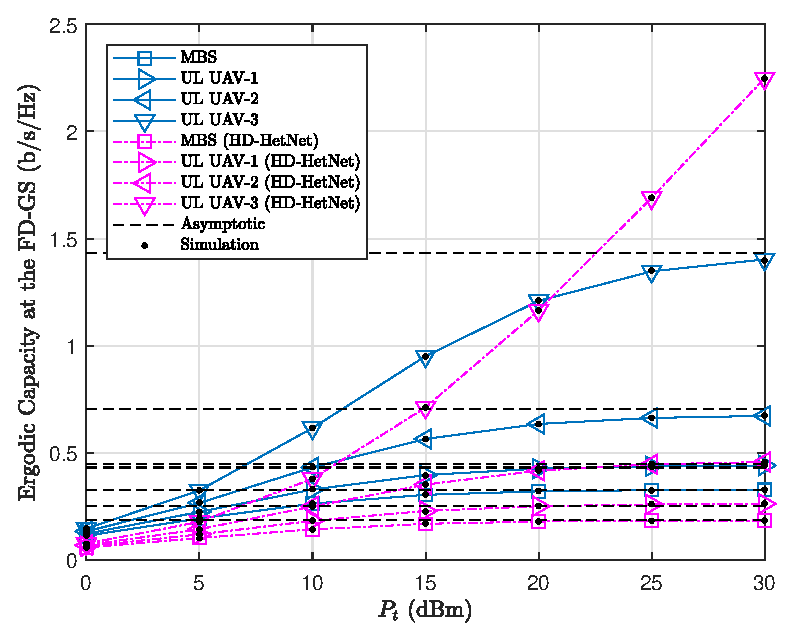
\includegraphics [width=0.45\columnwidth]{chap7_fig/FD_GS_capacity.eps}
\label{fig:NOMA_aided_multi_UAV_FD_HetNet_FD_GS_capacity}} \vspace{0cm}
\hfil
\subfloat[Ergodic Capacity at the DL UAVs.]{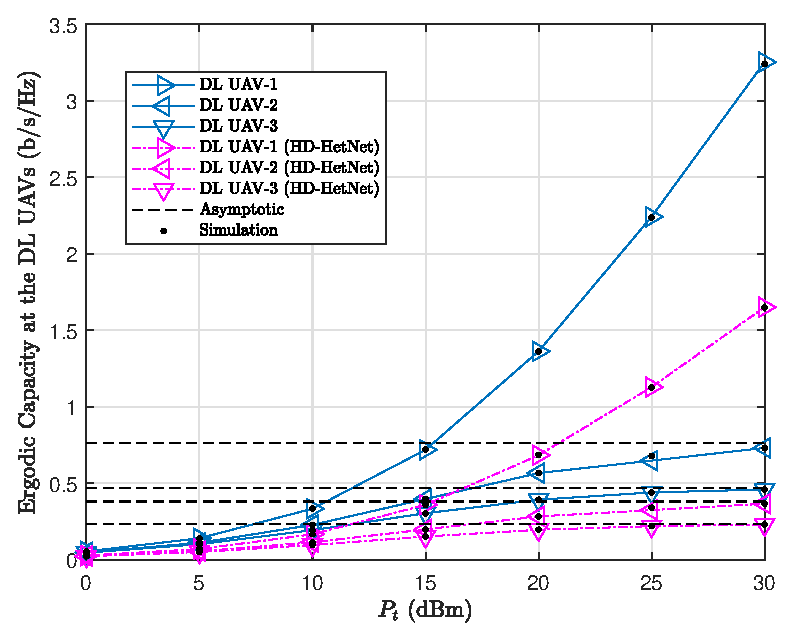
\includegraphics [width=0.45\columnwidth]{chap7_fig/DL_UAV_capacity.eps}
\label{fig:NOMA_aided_multi_UAV_FD_HetNet_DL_UAV_capacity}}
\caption{Ergodic capacity comparison at the FD-GS and DL UAVs in the NOMA-aided FD-HetNet for $N_U = N_D = 3$, $H_{min} = 0.1$ km, $\omega = 0.1$, $\gamma_{\phi}^2 = -130\text{ dBm}$, $\epsilon = 0.01$, and $\beta_{mbs,j} = \beta_{i,j} = (0.04)^3$.}
\label{fig:NOMA_aided_multi_UAV_FD_HetNet_erg_cap_fd_hetnet}
%\vspace{-1cm}
\end{figure*}

\begin{observation}
\emph{\emph{The MBS, UL UAVs, and DL UAVs deployed in the FD-HetNet attain higher ergodic capacity than the HD-HetNet.}}
\end{observation}

The ergodic capacity at the FD-GS is plotted in Fig. \ref{fig:NOMA_aided_multi_UAV_FD_HetNet_FD_GS_capacity} for the MBS $\big(C_{mbs}^{FD}\big)$ and UL UAV-$i$ $\big(C_{i}^{FD}\big)$. Likewise, the ergodic capacity at the DL UAVs $\big(C_{j}^{FD}\big)$ is plotted in Fig. \ref{fig:NOMA_aided_multi_UAV_FD_HetNet_DL_UAV_capacity}. As a benchmark, the ergodic capacities of the MBS $\big(C_{mbs}^{HD}\big)$, UL UAV-$i$ $\big(C_{i}^{HD}\big)$, and DL UAV-$j$ $\big(C_{j}^{HD}\big)$ are plotted for the NOMA-aided HD-HetNet.

Despite the FD-GS experiencing residual SI and MUI from the UL UAVs, it is observed from Fig. \ref{fig:NOMA_aided_multi_UAV_FD_HetNet_FD_GS_capacity} that $C_{mbs}^{FD}>C_{mbs}^{HD}$ and $C_{i}^{FD}>C_{i}^{HD}, i \in \{1,2\}$ for $0\text{ dBm} \leq P_t \leq 30\text{ dBm}$. Moreover, Corollaries \ref{NOMA_aided_multi_UAV_FD_HetNet_corollary_erg_cap_fd_noma_mbs} and \ref{NOMA_aided_multi_UAV_FD_HetNet_corollary_erg_cap_fd_noma_UL_uav_i} are confirmed, since $C_{mbs}^{FD} \approx C_{mbs,\infty}^{FD}$ and $C_{i}^{FD} \approx C_{i,\infty}^{FD}$ at high $P_t$ regimes. For the case of UL UAV-3, strong residual SI at the FD-GS is experienced at high $P_t$ regimes, leading to $C_{3}^{FD}<C_{3}^{HD}$. 

In Fig. \ref{fig:NOMA_aided_multi_UAV_FD_HetNet_DL_UAV_capacity}, it is observed that $C_{j}^{FD}>C_{j}^{HD}$ for $0\text{ dBm} \leq P_t \leq 30\text{ dBm}$. Furthermore, at high $P_t$ regimes, Corollary \ref{NOMA_aided_multi_UAV_FD_HetNet_corollary_erg_cap_fd_noma_DL_uav_j} is confirmed since $C_{j}^{FD} \approx C_{j,\infty}^{HD}, j \in \{2,3\}$. Specifically, it is observed that $C_{j}^{FD}, j \in \{2,3\}$ begins to plateau. Such a trend is due to the fact that the instantaneous SINR at DL UAV-$j, j \in \{2,3\}$, i.e., $SINR_j^{FD}$ becomes largely limited by MUI from the preceding $j-1$ DL UAVs, which cannot be canceled due to the nature of the SIC ordering. 

From Fig. \ref{fig:NOMA_aided_multi_UAV_FD_HetNet_erg_cap_fd_hetnet}, it is demonstrated that having the GS operate in FD mode, i.e., FD-HetNet, enables higher ergodic capacity over the HD-GS to be attained for the MBS, UL UAVs, and DL UAVs.

%%%%%%%%%%%%%%%%%%%%%%%%%%%%%%%%%%%%%%%%%%%%%%%%%%%%%%%%%%%%%%%%%%%%%%%%%%%%%%%%%%
% Effective SIC at the FD-GS and DL UAVs enables UAVs in the FD-HetNet to be deployed at lower altitudes with smaller altitude separation.
%%%%%%%%%%%%%%%%%%%%%%%%%%%%%%%%%%%%%%%%%%%%%%%%%%%%%%%%%%%%%%%%%%%%%%%%%%%%%%%%%%

\subsection{Impact of Height on Ergodic Sum Capacity}

\begin{figure}[h]
\centering \vspace{0.1cm}
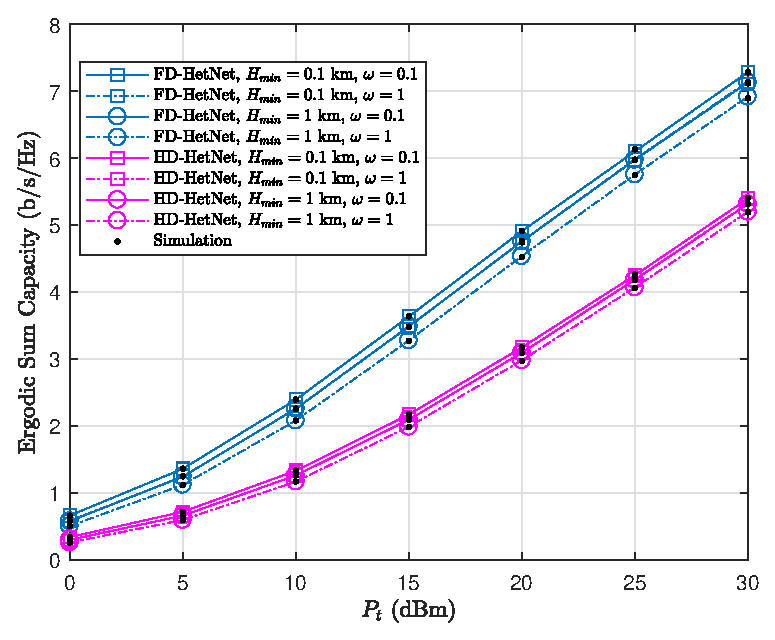
\includegraphics [width=0.45\columnwidth]{chap7_fig/height_impact_sum_capacity.eps}
%\vspace{-0.8cm}
\caption{Impact of height on the ergodic sum capacity of the NOMA-aided FD-HetNet and HD-HetNet for $N_U = N_D = 3$, $\gamma_{\phi}^2 = -130\text{ dBm}$, $\epsilon = 0.01$, and $\beta_{mbs,j} = \beta_{i,j} = (0.04)^3$.}
\label{fig:NOMA_aided_multi_UAV_FD_HetNet_height_impact_sum_capacity}
\end{figure}
%\vspace{-1cm}

\begin{observation}
\emph{\emph{The FD-HetNet attain higher ergodic sum capacity than the HD-HetNet when the altitude of the UAVs is increased.}}
\end{observation}

Fig. \ref{fig:NOMA_aided_multi_UAV_FD_HetNet_height_impact_sum_capacity} shows the impact of height on the ergodic sum capacity for the FD-HetNet and HD-HetNet. It can be seen that the ergodic sum capacity of the FD-HetNet $\big(C_{sum}^{FD}\big)$ and HD-HetNet $\big(C_{sum}^{HD}\big)$ exhibit similar trends, with $C_{sum}^{FD} > C_{sum}^{HD}$ for $0\text{ dBm} \leq P_t \leq 30\text{ dBm}$. When the minimum UAV altitude $\big(H_{min}\big)$ is low and the altitude separation factor $(\omega)$ is small, a higher $C_{sum}^{x}, x \in \{FD, HD\}$ is observed. Correspondingly, it is seen that a higher $H_{min}$ and larger $\omega$ leads to a lower $C_{sum}^{x}, x \in \{FD, HD\}$. 

To see the reasons behind such a trend, it is important to note that increasing $H_{min}$ causes the UL and DL UAVs to be operating at a higher altitude. In turn, the SOIs of UL UAV-$i$ and the GS become weaker at the receiving GS and DL UAV-$j$, respectively. Similarly, increasing $\omega$ results in a larger separating altitude \textcolor{black}{among} all UAVs, i.e., higher operating altitude for all UAVs, leading to weaker MUI at the FD-GS and the DL UAVs. However, a larger $\omega$ also leads to a weaker SOI at the receiving GS and DL UAVs. 

When SIC detection is employed at the GS and DL UAV-$j$, MUI from the UAVs can be effectively managed. Hence, both the FD-HetNet and HD-HetNet are able to have the UL and DL UAVs operate a lower $H_{min}$ and smaller $\omega$ while achieving higher $C_{sum}^{x}, x \in \{FD, HD\}$, leading to the trend in Fig. \ref{fig:NOMA_aided_multi_UAV_FD_HetNet_height_impact_sum_capacity}.

%%%%%%%%%%%%%%%%%%%%%%%%%%%%%%%%%%%%%%%%%%%%%%%%%%%%%%%%%%%%%%%%%%%%%%%%%%%%%%%%%%
% FD-HetNets can support more UAVs in NOMA-aided multi-UAV communications and is thus a viable solution to address spectrum scarcity.
%%%%%%%%%%%%%%%%%%%%%%%%%%%%%%%%%%%%%%%%%%%%%%%%%%%%%%%%%%%%%%%%%%%%%%%%%%%%%%%%%%

\subsection{Impact of the Number of Deployed UAVs on Ergodic Sum Capacity}

\begin{figure}[h]
\centering \vspace{0.1cm}
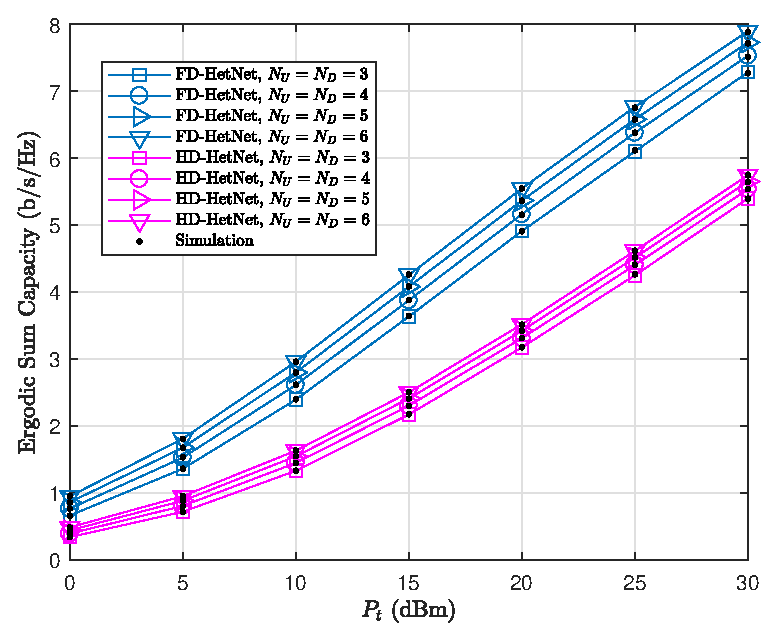
\includegraphics [width=0.45\columnwidth]{chap7_fig/number_deployed_UAVs_sum_capacity.eps}
%\vspace{-0.8cm}
\caption{Impact of the number of deployed UAVs on the ergodic sum capacity of the NOMA-aided FD-HetNet and HD-HetNet for $H_{min} = 0.1$ km, $\omega = 0.1$, $\gamma_{\phi}^2 = -130\text{ dBm}$, $\epsilon = 0.01$, and $\beta_{mbs,j} = \beta_{i,j} = (0.04)^3$.}
\label{fig:NOMA_aided_multi_UAV_FD_HetNet_number_deployed_UAVs_sum_capacity}
\end{figure}
%\vspace{-1cm}

\begin{observation}
\emph{\emph{Effective SIC at the GS and DL UAVs enables the FD-HetNet to attain higher ergodic capacity over the HD-HetNet.}}
\end{observation}

The impact of the number of deployed UAVs on the ergodic sum capacity for the FD-HetNet and HD-HetNet is plotted in Fig. \ref{fig:NOMA_aided_multi_UAV_FD_HetNet_number_deployed_UAVs_sum_capacity}. As SIC detectors are employed at the GS and DL UAVs, MUI from the UAVs can be effectively mitigated in the FD-HetNet and HD-HetNet. As a consequence, more UL and DL UAVs can be supported. Thus, increasing $N_U$ and $N_D$ leads to higher ergodic sum capacity $\big(C_{sum}^{x}, x \in \{FD, HD\}\big)$ for both FD-HetNet and HD-HetNet, as observed in Fig. \ref{fig:NOMA_aided_multi_UAV_FD_HetNet_number_deployed_UAVs_sum_capacity}. 

It is also useful to note that in HD-HetNets, the MBS and UL UAVs communicate on time-frequency resource blocks that are orthogonal to those allocated for DL UAVs. In contrast, the FD-GS enables the MBS, UL UAVs and DL UAVs to communicate over the same time-frequency resource block. As a result, increasing $N_U$ and $N_D$ leads to a higher increase in $C_{sum}^{FD}$ than in $C_{sum}^{HD}$, which in turn leads to $C_{sum}^{FD} > C_{sum}^{HD}$ for $0\text{ dBm} \leq P_t \leq 30\text{ dBm}$.

Therefore, Fig. \ref{fig:NOMA_aided_multi_UAV_FD_HetNet_number_deployed_UAVs_sum_capacity} highlights the potential for FD-HetNets to address spectrum scarcity in UAV communications.

%%%%%%%%%%%%%%%%%%%%%%%%%%%%%%%%%%%%%%%%%%%%%%%%%%%%%%%%%%%%%%%%%%%%%%%%%%%%%%%%%%
% High SI cancellation and UL interference management in the FD-HetNet is essential towards achieveing ergodic sum capacity that is greater than the HD-HetNet.
%%%%%%%%%%%%%%%%%%%%%%%%%%%%%%%%%%%%%%%%%%%%%%%%%%%%%%%%%%%%%%%%%%%%%%%%%%%%%%%%%%

\subsection{Impact of SI Cancellation, Phase Noise, and Residual Interference on Ergodic Sum Capacity}

\begin{figure}[th]
\centering \vspace{0.1cm}
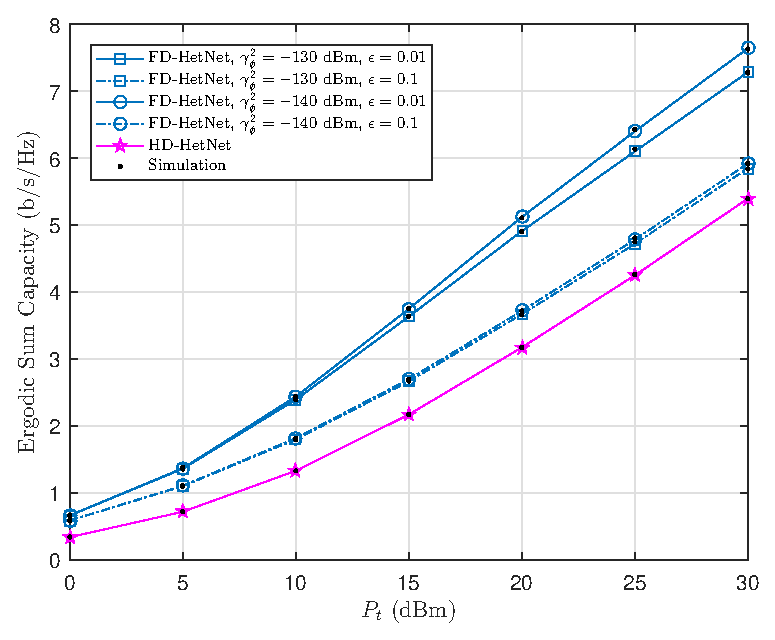
\includegraphics [width=0.45\columnwidth]{chap7_fig/phase_noise_epsilon_sum_capacity.eps}
%\vspace{-0.8cm}
\caption{Impact of SI cancellation and phase noise on the ergodic sum capacity of the NOMA-aided FD-HetNet for $N_U = N_D = 3$, $H_{min} = 0.1$ km, $\omega = 0.1$, and $\beta_{mbs,j} = \beta_{i,j} = (0.04)^3$.}
\label{fig:NOMA_aided_multi_UAV_FD_HetNet_phase_noise_epsilon_sum_capacity}
\end{figure}
%\vspace{-1cm}

\begin{observation}
\emph{\emph{The benefits of the considered FD-HetNet require SI cancellation of at least 137 dB. Such levels of SI cancellation have been reported in the literature.}}
\end{observation}

The impact of SI cancellation ($\epsilon$) and phase noise ($\gamma_{\phi}^2$) on the FD-HetNet ergodic sum capacity $\big(C_{sum}^{FD}\big)$ is shown in Fig. \ref{fig:NOMA_aided_multi_UAV_FD_HetNet_phase_noise_epsilon_sum_capacity}. To begin, it is useful to recall that SI cancellation is computed as $1/(\epsilon \sigma^2)$ \cite{ernest2019outage,zlatanov2017capacity}. Thus, increasing $\epsilon=0.01$ to $\epsilon 0.1$ also increases the SI channel estimation error while leading to a lower level of SI cancellation at the FD-GS. Consequently, the resultant instantaneous SINR of the MBS $\big(SINR_{mbs}^{FD}\big)$ and UL UAV-$i$ $\big(SINR_{i}^{FD}\big)$ at the FD-GS becomes limited by residual SI. Similarly, increasing $\gamma_{\phi}^2$ also causes the strength of the residual SI to increase. However, as $\gamma_{\phi}^2 < \sigma^2$, changes in $\epsilon$ have more significant impact on the FD-GS as the residual SI may be above the noise floor. Thus, as seen in Fig. \ref{fig:NOMA_aided_multi_UAV_FD_HetNet_phase_noise_epsilon_sum_capacity}, decreasing $\epsilon$, i.e., increasing SI cancellation, elicits a higher $C_{sum}^{FD}$ than reducing $\gamma_{\phi}^2$.

\begin{figure}[th]
\centering \vspace{0.1cm}
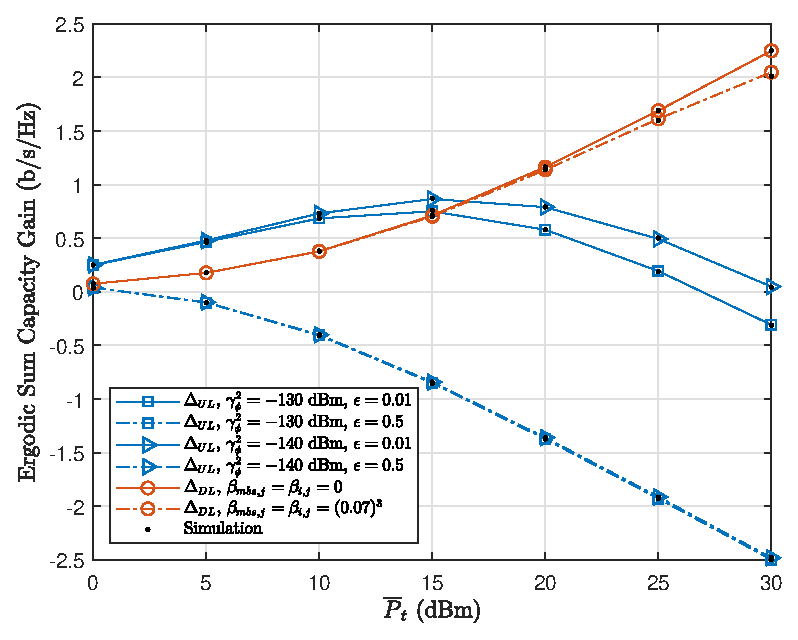
\includegraphics [width=0.45\columnwidth]{chap7_fig/ergodic_capacity_gain.eps} 
%\vspace{-0.8cm}
\caption{Impact of SI cancellation, phase noise, and residual interference on the ergodic sum capacity gain of the NOMA-aided FD-HetNet for $N_U = N_D = 3$, $H_{min} = 0.1$ km, and $\omega = 0.1$.}
\label{fig:NOMA_aided_multi_UAV_FD_HetNet_phase_noise_epsilon_residual_interference_sum_capacity}
\end{figure}
%\vspace{-1cm}

Fig. \ref{fig:NOMA_aided_multi_UAV_FD_HetNet_phase_noise_epsilon_residual_interference_sum_capacity} shows the impact of SI cancellation, phase noise, and residual interference $(\beta_{x,j}, x \in \{mbs, i\})$ on the ergodic capacity gain for UL and DL transmissions, i.e., $\Delta_{UL}$ and $\Delta_{DL}$. As explained earlier, increasing $\epsilon$ leads to a more drastic drop in $\Delta_{UL}$ than increasing $\gamma_{\phi}^2$, as seen in Fig. \ref{fig:NOMA_aided_multi_UAV_FD_HetNet_phase_noise_epsilon_residual_interference_sum_capacity}. Furthermore, a slight increase in $\beta_{mbs,j}$ and $\beta_{i,j}$ also leads to a drop in $\Delta_{DL}$ as the DL UAVs become limited by residual interference at high $P_t$ regimes. Therefore, Corollary \ref{NOMA_aided_multi_UAV_FD_HetNet_corollary_erg_cap_gain} is confirmed in Fig. \ref{fig:NOMA_aided_multi_UAV_FD_HetNet_phase_noise_epsilon_residual_interference_sum_capacity}.

It is worth emphasizing that the analysis in this chapter assumes SI cancellation levels of 137 dB $(\epsilon=0.5)$ to 154 dB $(\epsilon=0.01)$. Such SI cancellation levels have been reported in \cite{choi2013simultaneous}, where SI cancellation beyond 150 dB was noted. Therefore, Fig. \ref{fig:NOMA_aided_multi_UAV_FD_HetNet_phase_noise_epsilon_sum_capacity} and Fig. \ref{fig:NOMA_aided_multi_UAV_FD_HetNet_phase_noise_epsilon_residual_interference_sum_capacity} highlights the feasibility of achieving practical FD-HetNets for NOMA-aided multi-UAV communications.

\section{Chapter Summary} \label{NOMA_aided_multi_UAV_FD_HetNet_sec_conclusion}
NOMA-aided multi-UAV communications in FD-HetNets is proposed in this chapter as a pragmatic and attractive solution to address spectrum scarcity in UAV communications. Through an analysis of the ergodic capacity within a BPP-based stochastic geometry framework, it is shown that higher ergodic capacities are attained by the MBS and UAVs in the FD-HetNet. In addition, the FD-HetNet allows more UAVs to be at lower altitudes while achieving a higher ergodic sum capacity and ergodic capacity gains over HD-HetNets. Finally, it is demonstrated that NOMA-aided multi-UAV communications in FD-HetNets achieve higher ergodic sum capacity over HD-HetNets despite weaker SI suppression and stronger phase noise. Hence, the feasibility of addressing spectrum scarcity in UAV communications is highlighted.

Thus far, the performance analysis of multi-UAV networks has focused on the specific case of single-antenna UAVs and GSs. However, multi-antenna transmitters and receivers are more commonly used in practice to improve the diversity gain of wireless systems. One drawback of such multi-antenna transceivers stems from the fact that the communications channel may become correlated due to insufficient antenna spacing. To this end, the performance of a NOMA-aided multi-UAV network over correlated fading channels is studied in the next chapter.






